% Setup Document
\documentclass[11pt,a4paper]{report}
\usepackage[english]{babel}
\usepackage{polski}
\usepackage[utf8]{inputenc}
\usepackage[margin=3.5cm]{geometry}
\usepackage{graphicx}
\usepackage{hyperref}
\usepackage{gensymb} % for \degree
\usepackage{minted} % for \begin{figure}
% \usepackage[colorinlistoftodos,prependcaption,textsize=tiny]{todonotes}
\usepackage{amsmath} % for piecewise equations
\usepackage[hyphens]{xurl}
\usepackage{listings}
\usepackage{xcolor}
\usepackage{enumerate}
\usepackage{multirow}

\usepackage{subcaption}

% for \ceil
\usepackage{mathtools}
\DeclarePairedDelimiter{\floor}{\lfloor}{\rfloor}

\definecolor{codegreen}{rgb}{0,0.6,0}
\definecolor{codegray}{rgb}{0.5,0.5,0.5}
\definecolor{codepurple}{rgb}{0.58,0,0.82}
\definecolor{backcolour}{rgb}{0.95,0.95,0.92}

\lstdefinestyle{mystyle}{
    backgroundcolor=\color{backcolour},   
    commentstyle=\color{codegreen},
    keywordstyle=\color{magenta},
    numberstyle=\tiny\color{codegray},
    stringstyle=\color{codepurple},
    basicstyle=\ttfamily\footnotesize,
    breakatwhitespace=false,         
    breaklines=true,                 
    captionpos=b,                    
    keepspaces=true,                 
    numbers=left,                    
    numbersep=5pt,                  
    showspaces=false,                
    showstringspaces=false,
    showtabs=false,                  
    tabsize=2
}

\lstset{style=mystyle}




%% ------------------------------------------------------------------
\begin{document}
\thispagestyle{empty}

\begin{titlepage}
\begin{center}

\includegraphics[width=\textwidth]{Images/logo_AGH.jpg}\\

\bf{\sf{WYDZIAŁ FIZYKI I INFORMATYKI STOSOWANEJ}}\\[5mm]

\bf{\sf{KATEDRA ODDZIAŁYWAŃ I DETEKCJI CZĄSTEK}}\\[12mm]

\sf{\huge Projekt dyplomowy}\\[12mm] 

\sf{\Large Ecosystem simulation under Unity game engine\\[2mm]
Symulacja ekosystemu przy użyciu silnika Unity
}\\[40mm]
\end{center}
\sf{
\begin{tabular}{ll}
Autor: & Konrad Jakub Walas\\
Kierunek studiów: &	Informatyka Stosowana\\
Opiekun pracy: & dr inż. Bartłomiej Rachwał\\
\end{tabular}
}\\[10mm]
\begin{center}
\sf{Kraków, 2022}
\end{center}

%% ########################################################
\newpage
%% ########################################################
\end{titlepage}

% \todototoc
% \listoftodos

\tableofcontents

\chapter{Introduction} \label{chr:intro}

Radiation therapy is an important field of medical science. Due to its highly specialized nature, there are very few free, ready-made software tools for working with this topic. In addition, the materials that can be found online are usually specialized articles, often requiring additional fees to gain access. For this reason, any applications connected to this area, especially open-source ones, are a significant help for students and scientists associated with this field.

One of the common devices used in radiation therapy is the linear accelerator. Like any sophisticated medical equipment, these devices require regular calibration to maintain their precision and reliability. Calibration is essential, not only to ensure the accuracy of the radiation dose delivered to patients but also to meet rigorous safety standards and regulatory compliance.

This thesis addresses this problem by proposing open software tools to assist in the maintenance of linear accelerators by developing a web application with functionality related to the calibration of these devices. 

The collaboration with Damian Kubat, the head of the Department of Medical Physics at the National Institute of Oncology in Kraków, has led to the identification of the most significant challenges encountered during routine calibration of linacs. Consequently, two modules have been developed with the potential to address these challenges.

\section{Purpose}

This work aims to extend an existing web application with two modules:

\begin{itemize}
    \item Winston-Lutz test
    \item MLC leaves alignment analysis for compliance with the designed plan
\end{itemize}

Both modules provide tooling for the calibration of linear accelerators with multileaf collimators. Ready solutions for carrying out the Winston-Lutz test are already available on the web, for example, the Pylinac library for Python language \cite{pylinac}, and they were used to develop the corresponding module. However, as for the analysis of the collimator leaves alignment and compliance with the plan, no ready-made solutions were found during the research phase, therefore the presented solution was designed from scratch as part of the thesis.

\pagebreak

\section{Structure of the thesis} 

The thesis consists of five main parts, that span the next chapters: 

\begin{description}
    \item[Part I - Background]: Chapters 2, 3, 4
    
    Concepts and theory that are related to the scope of the thesis.
    
    \item[Part II - Module Definition]: Chapters 5, 6

    Logical description of created modules and used algorithms.
    
    \item[Part III - Implementation]: Chapters 7, 8

    Technical description of the application and used tools.
    
    \item[Part IV - Analysis]: Chapter 9
    
    Performed evaluations and their results.
    
    \item[Part V - Summary]: Chapter 10
    
    Conclusions and fields of applications.
    
\end{description}


\chapter{Theoretical background}
\section{Principles of ecosystem simulation}
\subsection{Ecosystem}
In general we can consider a \emph{System} as any phenomenon that has at least two separable components working together through some interaction. The system can be either structural or functional. Systems can consist of smaller systems, each component being system on their own thus any particular system is part of a hierarchy of other systems. Therefore there is need to define scope and limits in order to not miss any important environmental relationships but on the other hand not to be overwhelmed with irrelevant information. 

Ecological systems are larger systems of nature. That systems can begin with individual organism and expand toward greater complexity such as \emph{communities} or \emph{populations}. Communities, together with non-organic elements form \emph{ecosystems}. The definition is rather arbitrary, and there is no specific way of defining that system. In practice the boundaries are set by investigator, and all interactions and structures within that boundaries form an \emph{ecosystem}. Generally it contains some species like trees or dogs and components of landscape like terrain, lakes or cities. Very large continental-sized ecosystems with strong biotic continuity are called \emph{biomes}. 

Ecosystems are controlled by external and internal factors, such as climate, topography material or cyclic life and competition between species present in that system.
\cite{Hall_Day_1977}

\subsection{Modeling Ecosystem}
\label{modeling_ecosystem}
Model is abstract representation or simplification of an system that is used for studying and simulations. Models are simpler than real systems and have just the most important functional attributes of the real system. Modeling can be used to better understand real ecosystems and aid the conceptualization and measurement of real complex systems. Another use is to predict the consequences of an action that would be expensive, devastating, or difficult to accomplish in the real ecosystem, or just to see "what if". Complexity of nature is often overwhelming, therefore modeling is needed to fully understand it, however models must be checked frequently against real world to ensure that their representation is accurate, at least in areas that we are concerned about.

Two major types of ecological models are \emph{analytic models} and \emph{simulation models}. Both approaches are intended to  increase our understanding and prediction of ecosystems and their components, but in practice the two methods are used for completely different questions. With the analytical model we have more calculations and advanced mathematics, while with the simulation approach we use simpler mathematics, heuristic solutions and greater use of computers.

Analytic models are rather simple, often linear systems, that can be accurately described by a set of mathematical equations whose behavior is well-known. On the other hand, simulation models use numerical computations to solve problems that are impossible or impractical to solve with analytic approach. Simulation models are more widely used, and are generally considered more ecologically realistic, while analytic models are great for their explanatory power and conciseness.

\subsection{Lotka-Volterra equations}
Lotka-Volterra equations are also known as the predator-prey equations. They are a pair of first-order nonlinear differential equations. They are used to describe the dynamics of biological or ecological systems with two interacting species, one as predator and one as prey. The equations contains populations change through time and growth rates of the two populations.

\begin{equation}
    \frac{dx}{dt} = \alpha x - \beta xy,
\end{equation}
\begin{equation}
    \frac{dy}{dt} = \delta xy - \gamma y,
\end{equation}

where
\begin{itemize}
    \item $x$ is the number of prey;
    \item $y$ is the number of predators;
    \item $\frac{dy}{dt}$ and $\frac{dx}{dt}$ represent the instantaneous change rates of the two populations;
    \item $t$ represents time;
    \item $\alpha, \beta, \gamma, \delta$ are positive real parameters describing the interaction of the two species
\end{itemize}

\subsubsection{Lotka-Volterra model limitations}
\label{lotkaVolterraLimitations}
As this model is analytical one, it has its limitations: \cite{lotka_volterra_wiki}
\begin{enumerate}
    \item The prey population is able to find food at all times.
    \item Prey is the only food source for predators.
    \item The rate of change of population is proportional to its size.
    \item During the process, the environment does not change in favour of one species, and genetic adaptation is inconsequential.
    \item Predators and are always willing to eat prey.
\end{enumerate}

\subsubsection{Prey equation explanation}
Term $\alpha x$ represents growth in population. Growth is exponential, as prey has unlimited food supply.
Term $\beta xy$ on the other hand is the rate of predation upon prey. It is proportional to the rate at which they meet, and sizes of both populations, meaning that if either $x$ or $y$ is zero, then there will be no predation.

Interpretation of whole equation: the rate of change in prey's population is equal to its own growth rate minus rate at which it is prayed upon.

\subsubsection{Predator equation explanation}
Term $\delta xy$ represents growth in population, as it is rate of predation (different constant is used, because population growth is not is not necessarily equal to the rate at which prey is eaten).
Term $\gamma y$ corresponds to the loss rate of the predators, due to emigration or natural death of individuals. This leads to exponential decay when there is no pray to supply predators growth.

Interpretation of whole equation: the rate of change in predator's population is determined by rate it consumes prey minus death rate.

\subsubsection{Solutions to the equations}
\begin{figure}[H]
    \centering
    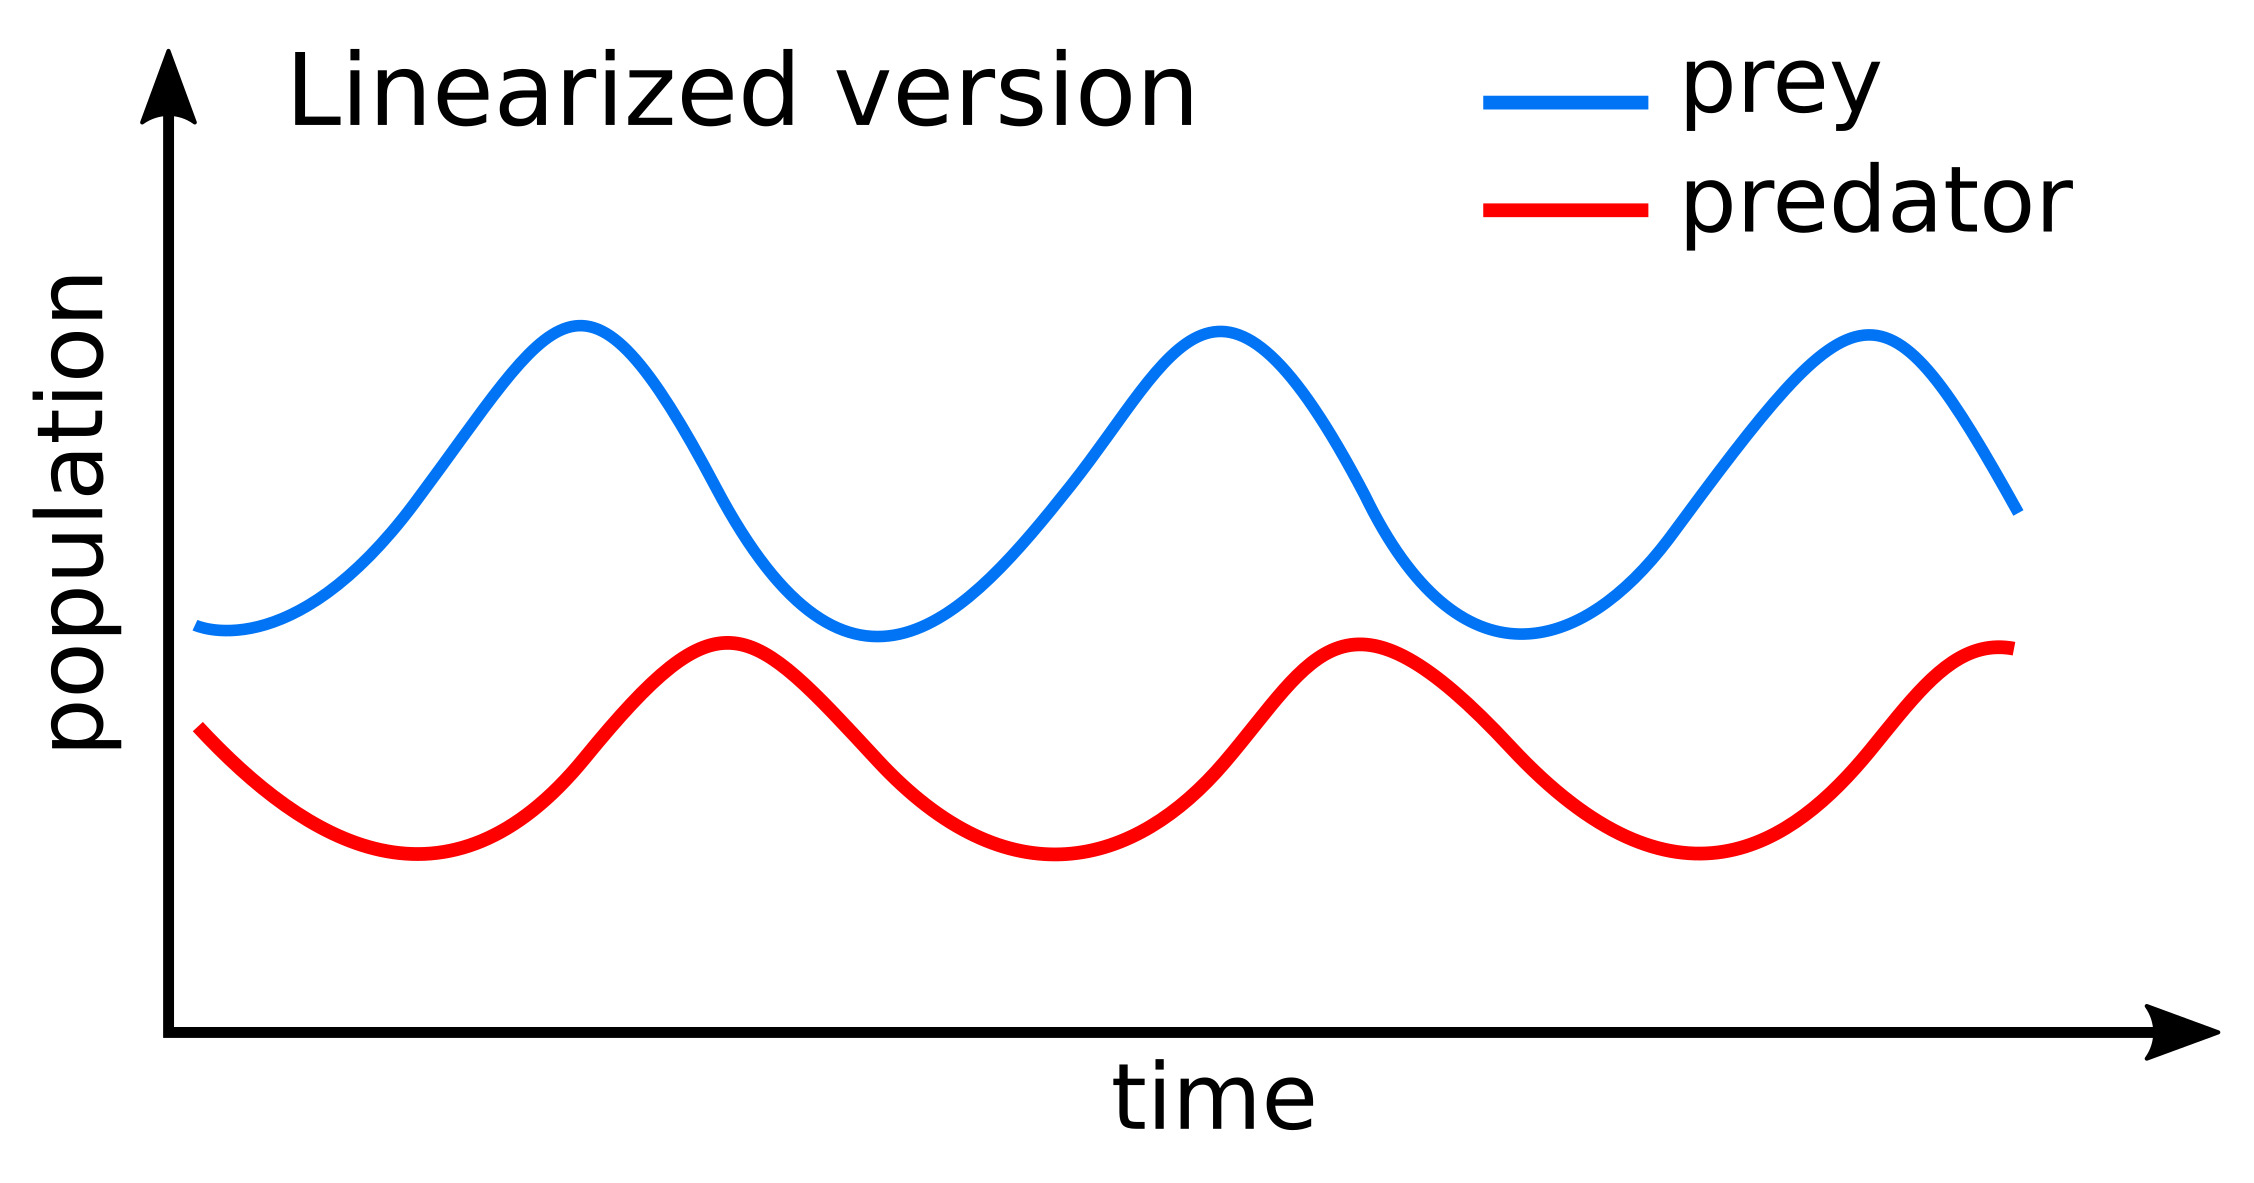
\includegraphics[width=0.6\textwidth]{Images/Lotka_Volterra_dynamics.jpg}
    \caption{Draft of solutions to Lotka-Volterra equations \cite{Lotka_Volterra_dynamics}}
    \label{fig:Lotka_Volterra_dynamics}
\end{figure}

Equations have periodic solutions with the population of predators trailing that of prey by $\pi/2$ in the cycle.
\\
\\
There are generalizations of the Lotka-Volterra equations, such as equations for n species or equations that include competition between those species \cite{BHARGAVA1989319}.

\section{Machine learning}
\emph{Machine Learning} is study of computer algorithms that are able to modify or adapt their actions through experience and use of data, so that these actions become more accurate. Machine learning is part of the broader topic of Artificial Intelligence.

When talking about machine learning it is good to define what learning actually is. The definition of \emph{learning} used in this thesis is getting better at some task through practice. This leads to question: how computer knows if it is getting better at some task. Answering that question provide a way to classify different algorithms int three main types:
\begin{enumerate}
    \item Supervised learning
    \item Unsupervised learning
    \item Reinforcement learning \cite{marsland_2015}
\end{enumerate}

Training using reinforcement learning was used in this thesis, so the focus is only on its description.

\subsection{Reinforcement Learning}
The goal of reinforcement learning is to learn a \emph{policy}. Policy is a mapping from \emph{observations} to \emph{actions}. An observation is what the agent can measure from its environment (all its sensory inputs) and an action is change to the configuration of agent. In other words agent makes decision based on inputs it receives (observations) and does something (actions).

The main element of reinforcement learning is the reward signal. Rewards allow the algorithm to train its policies, as they give feedback on whether the actions taken by the agent were appropriate or not. 

\subsubsection{Training}
Training this model involves taking some initially random action and then, based on the feedback from the reward, adjusting the probability of new actions so that they better fit the goal and receive a larger reward.

\begin{figure}[H]
    \centering
    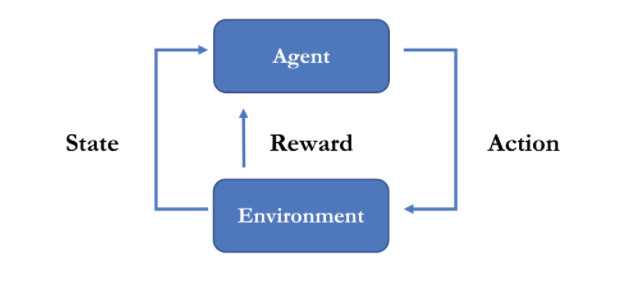
\includegraphics[width=\textwidth]{Images/rl_cycle.jpg}
    \caption{The reinforcement learning cycle. \cite{rlCycle}}
    \label{fig:rlCycle}
\end{figure}

\subsubsection{Curriculum learning}
Curriculum learning is a way of training a machine learning model where more difficult aspects of a problem are gradually introduced in such a way that the model is always optimally challenged.

\subsection{Observations and Sensors}
For an agent to learn, observations should contain all the information the agent needs to perform its task. Without sufficient and relevant information, the agent may learn poorly or may not learn at all. A reasonable approach to determining what information should be included is to consider what would be needed to compute an analytical solution to the problem, or what a human might be expected to be able to use to solve the problem. 

There can be many types of sensors, but the focus here is on two: \emph{vector sensor} and \emph{grid sensor}. A vector sensor is simply a vector of real values that are sent to the policy. The sensor uses a set of box queries in a grid shape and gives a top-down 2D view around the agent. During observations, the sensor detects the presence of detectable objects in each cell and encode that into one-hot representation. The collected information from each cell forms a 3D tensor observation and will be fed into the convolutional neural network of the agent policy (CNNs are a class of artificial neural networks that are most commonly used to analyze visual images). The observation for each grid cell is a one-hot encoding of the detected object. The total size of the created observations is $x_g \times\ y_g \times n$, where $x_g$ and $y_g$ are size of grid in each dimension and $n$ is number of elements that the agent can recognize. \cite{MLAgentsSensors}

\subsubsection{One-hot encoding}

In one-hot encoding, a separate bit of state is used for each state. It is called one-hot because only one bit is “hot” or TRUE at any time. \cite{harrisOneHot}

\subsection{The machine learning process}
There are some common steps for solving given problem using machine learning.
\begin{enumerate}
    \item Data Collection and Preparation
    \item Feature Selection
    \item Algorithm Choice
    \item Parameter and Model Selection
    \item Training
    \item Evaluation \cite{marsland_2015}
\end{enumerate}

\section{Genetic algorithms}
\emph{Genetic} algorithms are metaheuristics inspired by process of natural selection. They are a part of Evolutionary Computation which is one of the three pillars of Computational Intelligence (CI). The CI is the theory, design, application and development of biologically and linguistically motivated computational paradigms. \cite{what_is_ci}
Two other parts are Neural Networks and Fuzzy Systems. CI, and therefore genetic algorithms are used to develop systems, including games, in which agents behave intelligently.

There is no clear definition of genetic algorithms, but most methods that called GAs have following gears in common:
\begin{itemize}
    \item Population of chromosomes
    \item Selection according to fitness
    \item Crossover to produce new offspring
    \item Random mutation of new offspring
\end{itemize}

\subsection{Principles of Genetic Algorithms}
In a genetic algorithm, a population of candidate solutions is evolved toward better solutions (more information on what it means to find a better solution can be found later in this chapter). These solutions are called individuals, creatures or phenotypes. Each candidate has a set of properties, called \emph{genotype} or \emph{chromosomes}, that can be altered or mutated in order to evolve into better solution. There are many ways to represent a chromosome, but one of the most popular representations is a binary string of 0s and 1s. For problems involving numbers, these can be converted to their binary representation so that they can be used in this representation.

The algorithm usually starts with a population of randomly generated individuals. For each iteration, called a generation, fitness is calculated and inferior solutions are replaced by new ones from the best individuals. The new generation is used in the next iteration of the algorithm. In most cases, the algorithm terminates when the maximum number of generations is reached or when a satisfactory fitness level is reached.

\subsection{Fitness function}
The goal of GA used to solve optimization problems is to find a set of parameter values that maximize some specified, often multi-parameter function. This function is called \emph{fitness function}. In other words, the result of this function indicates how suitable a certain set of parameters, or \emph{chromosome}, is for solving a given problem. 

\subsection{Genetic Operators}
There are three common types of operators: selection, crossover, and mutation.
\begin{enumerate}
    \item \emph{\textbf{Selection}} This operator selects chromosomes in the population for reproduction. Chromosomes that has higher fitness are more likeky to be selected to reproduce (possibly several times).
    \item \emph{\textbf{Crossover}} In crossover one or more off-springs are produced using the genetic material of the parents. There are several types of crossover operator such as \emph{One Point Crossover}, \emph{Multi Point Crossover} or \emph{Uniform Crossover}. The simplest and one of the most commonly used is One Point Crossover, where one random crossover point is selected and the tails of the two parents are swapped to produce new offspring.
    \item \emph{\textbf{Mutation}} This operator randomly flips some of the bits in a chromosome. For example, the string 00000100 can be mutated at its second position, giving 01000100. Mutation can occur at each bit position in a string with some, usually very small probability like 0.001).
\end{enumerate}

\subsection{Simple genetic algorithm}
Most GAs (given a clearly defined problem and a bit string representation for candidate solutions) follow the following algorithm \cite{mitchell_1998}:

\begin{enumerate}
    \item Start with a randomly generated population of $n$ $l$-bit chromosomes (candidate solutions to a problem).
    \item Calculate the fitness $f(x)$ of each chromosome $x$ in the population.
    \item Repeat the following steps until $n$ offspring have been created:
    \begin{enumerate}
        \item Select a pair of parent chromosomes from the current population, the probability of selection being an increasing function of fitness. Selection is done "with replacement", meaning that the same chromosome can be selected more than once to become a parent.
        \item With probability $p_c$ (the "crossover probability" or "crossover rate"), cross over the pair at a randomly chosen point (chosen with uniform probability) to form two offspring. If no crossover takes place, form two offspring that are exact copies of their respective parents. (Note that here the crossover rate is defined to be the probability that two parents will cross over in a single point. There are also "multi-point crossover" versions of the GA in which the crossover rate for a pair of parents is the number of points at which a crossover takes place.)
        \item Mutate the two offspring at each locus with probability $p_m$ (the mutation probability or mutation rate), and place the resulting chromosomes in the new population.
        \item If $n$ is odd, one new population member can be discarded at random.
    \end{enumerate}
    \item Replace the current population with the new population.
    \item Go to step 2.


\end{enumerate}
\chapter{The project namespace}

\section{Logical items}
\begin{description}
    \item[Ecosystem] - consists of environment together with actors who can interact with themselves and with this environment and evolve over time.
    \item[(Ecosystem) Component] - the building block of ecosystem. Everything in the ecosystem is a component of the ecosystem.
    \item[Environment] - set of components that agent is able to perceive and interact with.
    \item[Interaction] - happens between two agents or other simulation object, is initiated by agent.
    \item[Action] - result of decision made by agent.
    \item[Agent] - entity that is able to move, make decisions and interact with its environment.
    \item[Food] - stationary object that can actor can interact with.
    \item[Environment element] - stationary object that agent can collide with.
\end{description}

\section{Technical items}
\begin{description}
    \item[Academy] - Singleton object which controls timing, reset, and training/inference settings of the environment.
    \item[Action] - The carrying-out of a decision on the part of an agent within the environment.
    \item[Agent] - Unity Component which produces observations and takes actions in the environment. Agents actions are determined by decisions produced by a Policy.
    \item[Decision] - The specification produced by a Policy for an action to be carried out given an observation.
    \item[Editor] - The Unity Editor, which may include any pane (e.g. Hierarchy, Scene, Inspector).
    \item[Experience] - Corresponds to a tuple of [Agent observations, actions, rewards] of a single Agent obtained after a Step.
    \item[External Coordinator] - ML-Agents class responsible for communication with outside processes (in this case, the Python API).
    \item[Frame] - An instance of rendering the main camera for the display. Corresponds to each Update call of the game engine.
    \item[Observation] - Partial information describing the state of the environment available to a given agent. (e.g. Vector, Visual)
    \item[Policy] - The decision making mechanism for producing decisions from observations, typically a neural network model.
    \item[Reward] - Signal provided at every step used to indicate desirability of an agent’s action within the current state of the environment.
    \item[State] - The underlying properties of the environment (including all agents within it) at a given time.
    \item[Step] - Corresponds to an atomic change of the engine that happens between Agent decisions.
    \item[Trainer] - Python class which is responsible for training a given group of Agents.  \cite{MLAgents_glossary}

\end{description}

\chapter{Ecosystem definition}
\label{ecosystemDefinitionChapter}

The current and the following chapters define the ecosystem model used in the rest of the thesis. This chapter focuses on passive side of model, what builds an ecosystem, and relationships between these components. \autoref{simulationChapter} provides a dynamic description of the model and what happens to the ecosystem when the passage of time is taken into account.

\section{Agents}
Agents are heart of the ecosystem, they are components that can do something, interact with other components and change state of ecosystem. 

There are two types of agents - prey and predators. Predators hunt prey, which feeds on plants.

Each agent have two sets of parameters - features and needs. Features alters agent's abilities and efficiency and needs influence decision making.

\subsubsection{Species}
Only agents of the same species can breed with each other. There are two species present in ecosystem:
\begin{enumerate}
    \item Rabbit
    
    The rabbit is a representative of the prey. Rabbits eat carrots, drink water, reproduce with other rabbits and avoid the foxes that hunt them. They usually have about 6 offspring in a litter, but that number can vary depending on parents.
    
    \item Fox
    
    The fox is a predator. They do not eat plants, but hunt rabbits, which are their main and only source of food. Foxes reproduce more slowly than rabbits and their typical number of cubs is 4.
\end{enumerate}

A more detailed description of agents, including their features, needs, and how they make decisions can be found in \autoref{agentsChapter}

\begin{figure}
    \centering
    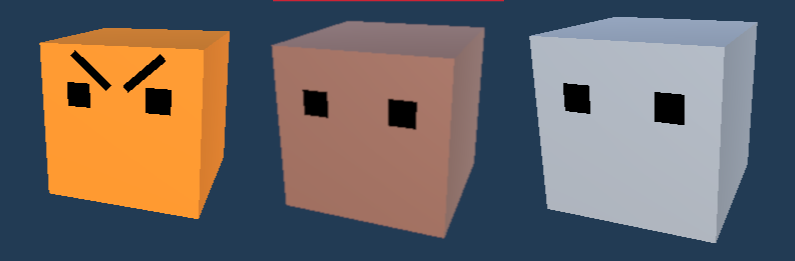
\includegraphics[width=\textwidth]{Images/agents.png}
    \caption{Graphical (GameObject) representation of agents used in Scene: fox, male rabbit and female rabbit.}
    \label{fig:agents}
\end{figure}

\section{Environment}
\subsection{Terrain}
The entire simulation takes place on a flat plane representing grass. There are two types of terrain in the environment - water and land. Agents cannot navigate through water, but they can satisfy their thirst near it. On land, individuals can move normally. 

\subsection{Food}
The environment contains food that is consumed by an herbivorous species. In this ecosystem there is only one species of plant - carrots. Carrots grow around certain points called \emph{Food Generators}. They appear at random points around the generator up to a certain number of plants, so new plants will only appear after the old ones have been eaten. 

The coordinates of a point $(x_f, y_f)$ in the Cartesian coordinate system relative to the generator position $(0, 0)$ are randomized and are represented by the following equation:

\begin{equation}
    x_f = r_f \cdot cos(\alpha)
\end{equation}
\begin{equation}
    y_f = r_f \cdot sin(\alpha)
\end{equation}
where
\begin{itemize}
    \item $r_f$ is random value in range $[0, r]$, $r$ is specific parameter defined in \hyperref[featuresNeedsStatesImplementation]{implementation}
    \item $\alpha$ is random angle in range $[0, 2\pi]$
\end{itemize}

Carrots grow over time, up to a certain maximum size. This is represented by growing in size. The longer a carrot lives, the larger it becomes and provides more energy to the individual who eats it. Carrots, unlike water, are consumed after being eaten by the rabbit, reducing its size. If the size is reduced below the minimum size, the carrot is considered to have been eaten whole and disappears from the ecosystem.

\begin{figure}
    \centering
    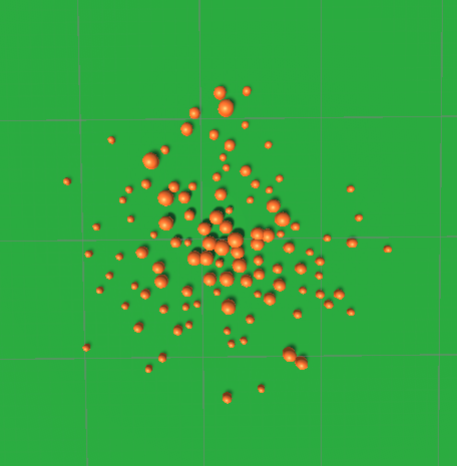
\includegraphics[width=\textwidth]{Images/carrot_generator_v2.png}
    \caption{Carrots around the generator with big maximum number of plants.}
    \label{fig:carrotGenerator}
\end{figure}

\subsection{Boundaries}
The ecosystem has specific dimensions. It is a square, with impassable barriers along its sides, beyond which agents cannot enter. Every element is located inside the boundaries.

\section{Interactions}
\label{interactionDescription}
Each interaction is initiated by an agent. There are two steps to initiate it. The agent must be ready to initiate the action, and then it must approach the object it wants to interact with. Interaction takes certain amount of time to complete and is different for each interaction, but interactions also can be instant. 

\subsubsection{Descriptions of each interaction}
Below you will find definitions of interactions between agents. A more detailed specification of these interactions, e.g. their duration, is included in \autoref{interactionsImplementationDescription}. A visual representation of interactions between agents can be found in \autoref{fig:interactionsDiagram}.
\begin{description}
    \item[Drinking] Happens between agents and water. Agent spend time near water satisfying thirst and at the end of interaction it reduces thirst by an amount proportional to the time spent drinking.
    \item[Mating] Happens between agents of the same species. Male agent need to find female partner that is willing to reproduce. If found partner do not have enough reproduction urge each interaction initiated by male agent will increase urge of its partner up to a point that mating can occur. New offspring are spawned at the end of interaction and new set of features is established through a genetic algorithm process. For more information, see \autoref{geneticAlgorithmsChapter}
    \item[Eating Carrot] Happens between rabbit and carrot. Similar to drinking agent spend some time near carrot and then reduces hunger by eaten amount. Here however carrot are consumed after interaction.
    \item[Eating Rabbit] Happens between fox and rabbit. Fox must find a rabbit and then eats it whole to reduce its hunger. Fox feeds one rabbit fully, reducing its hunger to zero.
\end{description}

\begin{figure}
    \centering
    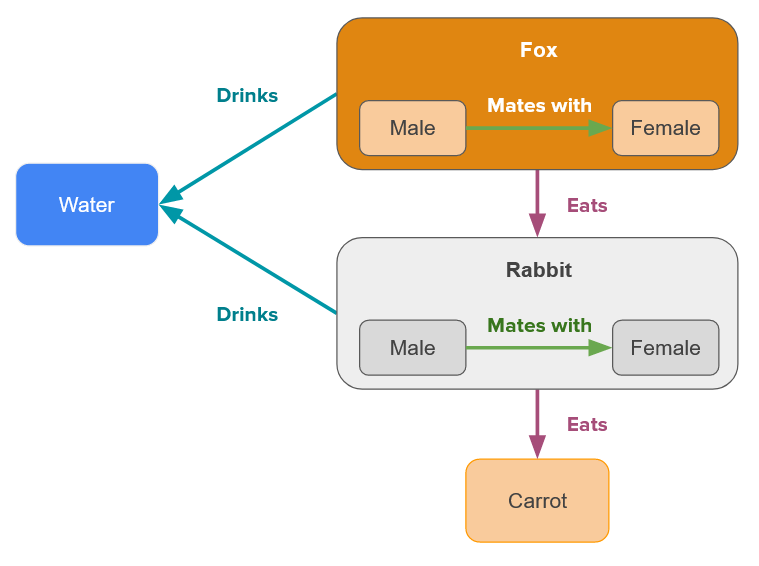
\includegraphics[width=\textwidth]{Images/interaction_diagram_v2.png}
    \caption{Diagram of interactions.}
    \label{fig:interactionsDiagram}
\end{figure}

\chapter{Simulation}
\label{simulationChapter}
\section{Simulation execution}
The simulation involves the execution of actions by agents present in the ecosystem. They take actions based on current needs and analysis of their environment. Each agent has the ability to make decisions, move and interact with the environment. Each agent focuses its actions to satisfy its needs. Needs increase in time, so each agent must meet them periodically. Rate at which needs are growing also depends on features - higher values means a better adapted individual, but it comes at a price in terms of faster energy consumption.

\section{Evolution of the simulation}
The purpose of the simulation is to observe evolution. Evolution occurs in the process of reproduction of individuals. Actors pass on their features to their offspring in the process of reproduction, thus increasing the population and diversity of the species. What is evolved is the set of features of the individuals. The model of movement and decision-making is not changed in any way. Therefore, individuals differ between generations only in features. During the simulation, both prey and predators evolve, developing their traits in parallel and adapting to the environment in which they live.

\section{Simulation metrics of interest}
During simulation various metrics are being tracked. These information is saved to file with timestamps but also are available live during simulation. User can navigate through the environment and display the current values of those metrics. Metrics observed during simulation:
\begin{itemize}
    \item Current population of rabbits
    \item Current population of foxes
    \item Median for each value of rabbits features 
    \item Median for each value of foxes features
    \item Number of rabbits dead for the following reasons: starvation, thirst, and being eaten by a fox
    \item Number of foxes dead for the following reasons: starvation, and thirst
\end{itemize}

\section{Advantages and disadvantages of the simulation model}
As being said in section \nameref{modeling_ecosystem} there are two ecological models that have different applications and restrictions.
There are some advantages to using this model due to fact that it bypasses some of the limits from the analytical model described in \nameref{lotkaVolterraLimitations}:
\begin{itemize}
    \item Prey is not always able to find food, it is determined by position of agent in 3D world and agents can die of starvation.
    \item During this process, agents evolve, changing their features and adapting to the environment. It depends on the particular simulation whether this adaptation favours one species or whether they evolve in parallel, effectively mitigating the impact of these changes on other species.
    \item Predators are not always willing to eat prey. They have other needs such as thirst and if they are not hungry, they will not hunt for prey.
\end{itemize}

However simulation has its own restrictions:
\begin{itemize}
    \item Simulation is non-deterministic. Due to the complexity of the models, interactions between them, and the randomness related to reproducing and inheritance, the state of the environment cannot be easily predicted. The outcome cannot be described by a function that depends only on time.
    \item Result does not necessarily have to be stable. Function of population over time will not always be periodical. It may happen that after several cycles one species suddenly goes extinct.
\end{itemize}
\chapter{The agent component details}
\label{agentsChapter}
This chapter is focused on a more detailed description of the agent. Agents are treated as a separate system with multiple components.

\section{Description of agent's components}
\subsection{Features}
\label{featuresDefinition}
\emph{Feature} is an integer ranging from 0 to 100. Features are set at agent's birth and are later unchangeable. Features alter agents parameters and have an impact on its behaviour. There are 3 features for each actor:
\begin{description}
    \item[Speed] alters agent's movement speed.
    
    \begin{equation}
        s = (\sqrt[50]{2})^{v-50} \cdot a_s
    \end{equation}
    where
    \begin{itemize}
        \item $s$ is agents movement speed
        \item $v$ is value of speed feature
        \item $a_s$ is specific parameter defined in \hyperref[featuresNeedsStatesImplementation]{implementation}
    \end{itemize}
    
    \item[Sensory Range] corresponds to agent ability to see other agents. For rabbits greater sensory range means that they can earlier begin to escape its predator.
    
    \begin{equation}
        r_s = \frac{r_{max} - r_{min}}{100} v + r_{min}
    \end{equation}
    where
    \begin{itemize}
        \item $r_s$ is agents sensory range
        \item $r_{min}$ is minimal sensory range
        \item $r_{max}$ is maximal sensory range
        \item $v$ is value of sensory range feature
    \end{itemize}
    
    \item[Fertility] is responsible for controlling how fast agent regenerates after reproduction
    
    \begin{equation}
        m = \frac{2}{500} v + 0.8
    \end{equation}
    where
    \begin{itemize}
        \item $m$ is modifier applied to growth rate of Reproduction urge of agent
        \item $v$ is value of fertility feature
    \end{itemize}
    
    Fertility also regulates how many offspring a mother gives birth to.
    
    \begin{equation}
        n = \bigg\lfloor {\frac{2d+1}{101} v} \bigg\rfloor - d
    \end{equation}
    where
    \begin{itemize}
        \item $n$ is the number of offspring a mother gives birth to
        \item $d$ is the maximum variation in the number of offspring by feature
        \item $v$ is value of fertility feature
    \end{itemize}
    
\end{description}

\subsubsection{Genetic cost}
The \emph{genetic cost} parameter $\delta$ is related to features. The higher values are, the better agent is adapted to the environment, but it does involve increased energy consumption. 

The genetic cost is simply the sum of all feature values.

\begin{equation}
    \delta = \sum_{i=1}^{n} v_i
\end{equation}
where
\begin{itemize}
    \item $v_i$ are value of i-th feature
    \item $n$ is number of features, in this case $n=3$
\end{itemize}

More useful, however, is the \emph{relative genetic cost} $\delta_r$, which is the ratio of the genetic cost to the sum of the maximum values of the traits.

\begin{equation}
    \delta_r = \frac{\delta}{n \cdot v_{max}} 
\end{equation}
where
\begin{itemize}
    \item $v^i_{max}$ are maximal value of i-th feature, in this case $v_{max} = 100$
    \item $n$ is number of features, in this case $n=3$
\end{itemize}

\subsection{Needs}
\label{needsDefinition}
\emph{Need} is a real number between 0 and 100. Needs are constantly increasing during the simulation. There are needs that must be satisfied for an agent to live, such as hunger, and if this need reaches its maximum value, the agent dies. Needs do not change any of the agent's parameters, but they influence the agent's decisions in such a way that the agent strives to satisfy them. There are 3 needs for each actor:
\begin{description}
    \item[Hunger] obliges agent to look for food or hunt for prey. If an agent's hunger reaches 100\% the agent dies.
    \item[Thirst] compels agent to look for water source and drink. If an agent's thirst reaches 100\% the agent dies.
    \item[Reproduction urge] pushes agent to look for mate and extend the species.
\end{description}

\subsubsection{Growth rate}
Rate at which needs grow is influenced by relative genetic cost up to two times the normal growth and can be described by function:

\begin{equation}
    f(t) = \alpha t (1 + \delta_r) \cdot m
\end{equation}
where
\begin{itemize}
    \item $f(t)$ is value of need at time t
    \item $\alpha$ is fixed need gain defined during simulation
    \item $\delta_r$ is relative genetic cost and $0 < \delta_r < 1$
    \item $m$ is modifier that can be different for each need, but is equal to $1$ in most cases
\end{itemize}

\subsection{Body}
Each agent has a body, which is responsible for the agent's physics. It has a collider and interacts with other objects in the game in a physical way.

\subsection{State Machine}
\emph{State Machine} is component responsible for deciding what activity should agent perform at given time, and activate relevant policy based on the surrounding environment and agent's needs.

\subsection{Machine Learning Agent}
A \emph{machine learning agent} is a subsystem of an agent that utilises machine learning. It is responsible for carrying out the activity determined by the state machine.

\subsubsection{Sensors}
The agent has two types of sensors:
\begin{enumerate}
    \item \textbf{Vector sensor}
    
    A vector sensor of agent consists of two elements: x-coordinate and y-coordinate of the agent's velocity vector.
    
    \item \textbf{Grid sensor}
    
    The agent has two grid sensors - one precise and the other long-range. The precise sensor is used by the agent to observe the agent's immediate surroundings and represents the agent's sense of sight, or hearing. The agent uses it to determine the exact location of environmental elements in its proximity. The long-range sensor, on the other hand, is responsible for the agent's general understanding of the environment and helps the agent determine the direction in which an environmental item is located without giving the agent its exact location. It represents the sense of smell, or again hearing.
     
    \textbf{Detectable components}: female fox, male fox, female rabbit, male rabbit, water, wall, food
     
\end{enumerate}

\subsubsection{Decision requester}
\emph{Decision requester} is component that request decision from policy automatically and periodically, at specified intervals. If decision is requested policy gathers input and maps it to actions. If the decision frequency is lower than the number of simulation frames, the last decision is repeated between frames.

\section{Decision making process}
The agent makes decisions based on observations of his environment, and his current needs. Observing the environment means, for example, spotting a predator, while deciding on the basis of current needs implies switching to food search mode when the agent is hungry. 

There are several pre-trained models of agent behaviour. Each model corresponds to some specific activity that the agent performs, for example searching for food. The choice of a particular model depends on the state the agent is in and is managed by a state machine.

Because training such a general model would be demanding and difficult to achieve, several less complex machine learning models are used, instead of a single, complex one handling the whole agent behaviour. The agent adapts its behavioural model to the current situation.

\subsubsection{Example}
The rabbit is very hungry and a bit thirsty. So the food-seeking state is activated, and thus the policy responsible for this task is loaded. After a while, the rabbit has found and eaten a carrot, but in the meantime its thirst has increased even more, so the state machine will switch on the state of searching for water. However, in the meantime, a fox has appeared next to the agent, so instead the state of running away from the predator will be activated. Until the rabbit either does not flee from the fox or is eaten this state will persist and the model responsible for fleeing will direct the agent's actions.

\subsection{Switching between states}
\label{switchingStates}
The states are selected on a ranking basis. The state machine constantly monitors all states in real time and selects the one with the highest rank. There are two types of states: \emph{main state} and \emph{special state}. 

The main states have ranking functions that determine the rank for a given state returning a real value $y \in [0, 1]$ . This function must be defined separately for each state. An example would be a linear function mapping the hunger value to the rank for the looking for food state.

Special states instead of a ranking function have an activation function returning the value $y \in \{0, 1\}$, and having a predetermined rank value from the range $[0, 2]$, which is multiplied by the value returned by the activation function.

\subsection{States}
\label{statesDefinition}
\subsubsection{Main States}
\begin{enumerate}
    \item \textbf{Chilling}
    
    Agents: all agents
    
    Description: This state represents agent's resting and is activated, when agent has nothing to do (all needs are met, there is no predator in sensory range).
    
    Ranking function:
    \begin{equation}
        f(x) = a_c
    \end{equation}
    where $a_c$ is specific parameter defined in \hyperref[featuresNeedsStatesImplementation]{implementation}.
    
    ML Model: Basic, untrained model, which means that the agent makes small random movements, but stays in one place at the same time without standing completely still.
    
    \item \textbf{Looking for food}
    
    Agents: rabbits
    
    Description: This state represents looking for carrots and is activated, when rabbit is hungry.
    
    Ranking function:
    \begin{equation}
        f(x) = x
    \end{equation}
    where $x$ is value of hunger.
    
    ML Model: \hyperref[eatingCarrotModel]{Eathing Carrot Model}
    
    \item \textbf{Hunting}
    
    Agents: foxes
    
    Description: This state represents looking for rabbits to eat and is activated, when fox is hungry.
    
    Ranking function:
    \begin{equation}
        f(x) = x
    \end{equation}
    where $x$ is value of hunger.
    
    ML Model: \hyperref[huntingModel]{Hunting Model}
    
    \item \textbf{Looking for mate}
    
    Agents: all agents
    
    Description: This state represents looking for partner to reproduce and is activated, when agent has high reproduction urge.
    
    Ranking function:
    \begin{equation}
        f(x) = \frac{x}{100}a_m^{x-100}
    \end{equation}
    where $x$ is value of reproduction urge and $a_m$ is specific parameter defined in \hyperref[featuresNeedsStatesImplementation]{implementation}.
    
    ML Model: \hyperref[matingModel]{Mating Model}
    
    \item \textbf{Looking for water}
    
    Agents: all agents
    
    Description: This state represents looking for water and is activated, when agent is thirsty.
    
    Ranking function:
    \begin{equation}
        f(x) = x
    \end{equation}
    where $x$ is value of thirst.
    
    ML Model: \hyperref[drinkingModel]{Drinking Model}
    
\end{enumerate}

\subsubsection{Special States}
\begin{enumerate}
    \item \textbf{Drinking}
    
    Agents: all agents
    
    Description: This state represents drinking and is active while agent is interacting with water.
    
    Activation function:
    \begin{equation}
        f(x)= \begin{cases} 
            0 \quad & \text{if drinking interaction is not active} \\
            1 \quad & \text{if drinking interaction is active}
          \end{cases}
    \end{equation}

    ML Model: None. Agent waits for drinking interaction to end.
    
    \item \textbf{Eating}
    
    Agents: rabbits
    
    Description: This state represents eating and is active while agent is interacting with carrot.
    
    Activation function:
    \begin{equation}
        f(x)= \begin{cases} 
            0 \quad & \text{if eating carrot interaction is not active} \\
            1 \quad & \text{if eating carrot interaction is active}
          \end{cases}
    \end{equation}

    ML Model: None. Agent waits for eating carrot interaction to end.
    
    \item \textbf{Escaping Predator}
    
    Agents: rabbit
    
    Description: This state represents running away from predator, when it is near.
    
    Activation function:
    \begin{equation}
        f(x)= \begin{cases} 
            0 \quad & \text{if no predator is in sensory range} \\
            1 \quad & \text{if predator is in sensory range}
          \end{cases}
    \end{equation}
    
    ML Model: \hyperref[escapingPredatorModel]{Escaping Predator Model}
    
\end{enumerate}

\subsection{Models}
The agent uses machine learning to make decisions about specific activity. For each of these actions, there is a different model responsible for solving that task.
\begin{enumerate}
    \item \textbf{Drinking}
    \label{drinkingModel}
    
    Description: Agent aims to find water as soon as possible and interact with it.
    
    \item \textbf{Eating Carrot}
    \label{eatingCarrotModel}
    
    Description: Agent aims to find carrot as soon as possible and interact with it.
    
    \item \textbf{Mating}
    \label{matingModel}
    
    Description: Agent aims to find carrot as soon as possible and interact with it.
    
    \item \textbf{Hunting}
    \label{huntingModel}
    
    Description: Fox aims to find rabbit as soon as possible and interact with it.
    
    \item \textbf{Escaping Predator}
    \label{escapingPredatorModel}
    
    Description: Rabbit aims to escape predator and avoid being eaten.
    
\end{enumerate}

\newpage
\subsection{Actions}
\emph{Actions} are results of agent decisions. Essentially actions are values returned by policy that tells agent how to behave. Actions can be discrete or continuous. In this simulation all agents have the same actions - three continuous actions and one discrete action.

\subsubsection{Continuous actions}
\begin{itemize}
    \item value telling agent to move forward or backward,
    \item value telling agent to move right or left,
    \item value by which agent should rotate.
\end{itemize}

Each continuous action has value in range $[-1, 1]$.

\subsubsection{Discrete actions}
\begin{itemize}
    \item boolean value to tell if agent want to initiate interaction.
\end{itemize}
\chapter{Genetic algorithms for evolution of agents}
\label{geneticAlgorithmsChapter}
In the same way that a simulation model of an ecosystem differs from an analytical one, the different parts of the genetic algorithm used in this simulation will also differ slightly compared to standard genetic algorithms.

\section{Selection}
Firstly, there is no defined fitness function. It is not needed. During the simulation, the individuals match naturally. If an individual is less well adapted to its environment, there is a greater chance that it will be eaten or that it will not be able to satisfy its own needs and will die. The individuals who do mate, however, are those who have managed to overcome difficulties. They are able to pass on to their offspring the genes that have enabled them to get this far. Selection can thus be referred to as natural selection.

\section{Chromosome representation}
Naturally, a chromosome will correspond to the set of all traits an agent possesses and a single gene to a single trait.

\section{Crossover}
As the number of offspring is usually greater than 2, uniform crossover has been chosen as the crossover operator. During gene passing, it is randomly determined whether a child receives a feature from its father or its mother. The probabilities are each equal to 0.5.

\section{Mutation}
As chromosome contains integer values random resetting mutation method was chosen. For each gene (feature), there is a probability that it will be replaced by a new random integer value $v \in [0, 100]$.
\chapter{Implementation in Unity Engine}
This chapter describes how the theoretical model described in the previous chapters has been implemented in practice, detailing the specific parameters defined previously.

In addition, due to its technical nature, the nomenclature from Unity engine \cite{UnityGlossary} will be used, in particular:

\begin{description}
    \item[GameObject] - used to represent everything which can exists in scene. Every object in game is GameObject. GameObject contains components.
    \item[Prefab] - The Prefab Asset acts as a template from which new Prefab instances (GameObjects) can be created in the Scene
    \item[Component] - object that define properties and behaviour of GameObject it is attached to.
\end{description}
Project and the source code can be found in public repository on GitHub:
\url{https://github.com/kerdamon/Engineering-Thesis-Simulating-Ecosystem}

\section{Components}
Below is the list of custom components written for the project:

\begin{enumerate}
    \item State machine - handling state change described in \autoref{switchingStates}
    \item Interactions - handling interactions described in \autoref{interactionDescription}
    \item Interaction managers - handling the initiation of the corresponding interaction when an agent wants to initiate it and the appropriate conditions are met
    \item Agent component - handling training and inference of ML model
    \item Simulation Control - gathering statistics during simulation
    \item Training Area managers - controlling training environment, for example, provides the ability to place agents in a random position in a training environment
    \item Food managing - components used to control plant growth
    \item Needs - managing needs of agent
    \item Features - managing features of agent
\end{enumerate}
As the thesis does not focus on a strictly technical approach to the problem, it is not necessary to describe most of the components, except for the description interactions and values of parameters for features, needs and sates in order to make their functioning more precise.

\subsection{Interactions}
\label{interactionsImplementationDescription}
Below are specific values of parameters regulating the functioning of the interactions defined in \autoref{interactionDescription}

\subsubsection{Drinking Interaction}
\begin{description}
    \item[Max drinking time] - after this time agent regenerates max thirst: 10 s
    \item[Step time] - determines the minimum time to record drinking progress: 0.5s
    \item[Regeneration per step] - amount by which thirst changes in each step: 5
\end{description}

\subsubsection{Mating Interaction}
\begin{description}
    \item[Duration time]: 5 s
\end{description}

\subsubsection{Eating Carrot Interaction}
\begin{description}
    \item[Max eating time] - after this time agent regenerates max hunger: 10 s
    \item[Step time] - determines the minimum time to record eating progress: 1s
    \item[Regeneration per step] - amount by which hunger changes in each step: 10
\end{description}

% \subsection{Features}
% \label{featuresImplementationDescription}
% Below are the specific values of the parameters described in the definition of features in \autoref{featuresDefinition}
% \begin{description}
%     \item[Speed] $a_s = 1$
%     \item[Sensory range] $r_{min} = 15, r_{max} = 27$
%     \item[Fertility] $d = 3$
% \end{description}

% \subsection{Needs}
% \label{needsImplementationDescription}
% Below are the specific values of the parameters described in the definition of needs in \autoref{needsDefinition}
% \begin{description}
%     \item[Growth rate] $\alpha = 0.5$
% \end{description}

% \subsection{States}
% \label{statesImplementationDescription}
% Below are the specific values of the parameters described in the definition of the states in \autoref{statesDefinition}
% \begin{description}
%     \item[Chilling] $a_c = 0.6$
%     \item[Looking for mate] $a_m = 1.01$
% \end{description}

\subsection{Features, needs and states}
\label{featuresNeedsStatesImplementation}
Below are the specific values of the parameters described in the definition of features, needs and states (subsections \ref{featuresDefinition}, \ref{needsDefinition} and \ref{statesDefinition}).
\begin{center}
    \begin{tabular}{ |c|c|c| } 
        \hline
        Name & Symbol & Value \\
        \hline \hline
        Speed coefficient & $a_s$ & 1 \\
        \hline
        Minimal sensory range & $r_{min}$ & 15 \\
        \hline
        Maximal sensory range & $r_{max}$ & 27 \\ 
        \hline
        Offspring variation by feature & $d$ & Rabbits: 3 \\
        &  & Foxes: 2 \\ 
        \hline
        Growth rate & $\alpha$ & 0.5 \\ 
        \hline
        Chilling coefficient & $a_c$ & 0.6 \\ 
        \hline
        Mating coefficient & $a_m$ & 1.01 \\ 
        \hline
    \end{tabular}
\end{center}



\section{Prefabs}
\subsubsection{Simulation and training Areas}
Areas contain agents together with environment. Each area contains terrain - plane, boundaries, water, food generators, rabbits and predators.

\begin{figure}
    \centering
    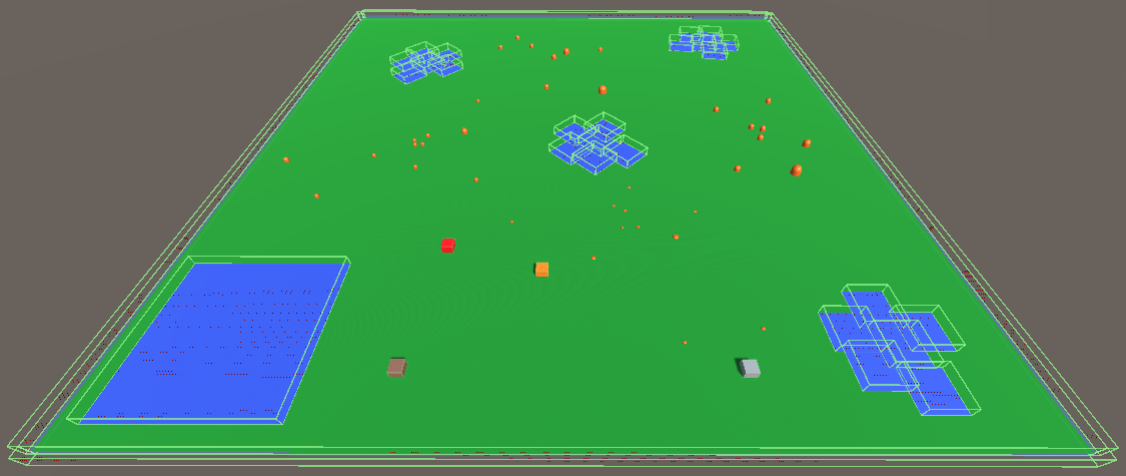
\includegraphics[width=\textwidth]{Images/simulation_area.png}
    \caption{Simulation area in Unity editor.}
    \label{fig:simulationArea}
\end{figure}

\subsubsection{Agents}
An agent is just an implementation of the agent defined in \autoref{agentsChapter}. 
The agent's body is a cube with side length 1. The agent also has a cubic collider which is used to initiate interactions with side length $1.5$, so it does not need to directly touch the body of the object it wants to interact with. 

Precision grid sensor has dimensions of 37 x 40 and a cell size of 1.5. Long-range grid sensor has dimensions of 20 x 20 and a cell size of $40$. The sensor has such a large range because, due to technical limitations, the smallest possible size of this sensor is 20x20, and the cell size had to be chosen so as not to give the agent the exact position of the object, only its general location.

The rabbit can give birth to a base of 6 offspring, the discrepancy due to fecundity is 3, while randomness can modify the number of offspring by 2. Thus, the final number of offspring the rabbit can give birth to is 1-11. For the fox, these numbers are 4, 2, and 1, respectively, giving a final number of offspring of 1 - 7. The probability of mutation is 0.005.

\subsubsection{Plant Generator and Carrots}
The carrot is a capsule of size 1, although it is modified according to the growth level of the plant. Its minimum size is 0.5, maximum is 1.5, and during growth it changes by 0.1 every 5 seconds. For the Plant Generator, the spawn range is 8, the spawn radius is equal to 6, and the plant limit is 15, but these parameters may vary depending on the simulation.

\subsubsection{Water}
Water is just a plane with a collider placed above its surface to allow sensors to detect it and to prevent agents from moving through the water. The base size of the water element is 5x5, while the sea element is 20x20. The lake element consists of 6 merged water elements.

\section{Scenes}
The project was divided into 6 scenes. Five of them are training scenes and one is a simulation scene. The training scenes are slightly modified versions of the simulation scene for purposes of training ML models. Each training scene contains multiple training areas specific to each model in order to train it better and faster. The base size of the plane is 200x200. 

Each scene contain main camera, lighting, event system (used for inputting keys) and area with environment and agents.

\subsubsection{Simulation scene layout}
Area present in this scene contains agents with with normal setup and behaviour with all states, models and interactions defined in \autoref{ecosystemDefinitionChapter} and \autoref{agentsChapter} and further specified above in this chapter.
Simulation scene also includes simulation controller GameObject responsible for measuring statistics during simulations and logging it, as well as canvas GameObject for displaying it on screen.

\subsubsection{Training scene layout}
The area present in this scene contains agents with modified states, interactions and simplified behaviours tailored to the specific model being trained. For example, in the mating training scene, the agents use a simplified mating interaction in which the male only needs to find a female and interact with her, after which the female is moved to a new random position and the male continues to search for a mate. There are also several copies of areas in the scenes to speed up the training of the model.

\begin{figure}
    \centering
    \includegraphics{Images/scene_layout_combined.png}
    \caption{Simulation and training scene layouts.}
    \label{fig:sceneLayout}
\end{figure}

The individual training scenes are described in more detail in \autoref{trainingEnvironmentsDescription}
\chapter{Training Models}
\label{trainingEnvironmentsDescription}
Training was done in following order: Drinking, Eatting Carrot, Mating, Hunting, Escaping Predator. Subsequent training scenarios are more and more advanced and use models that have been trained before. In each case, the agents' features are randomised so that the trained model could cope with the changing features during the simulation. Each scenario also had specific simplified interactions to aid the training process. Additionally, in the scenarios, the actors receive negative rewards that increase over time, accumulating to specific values intended to encourage the agents to complete the task as quickly as possible and not to sit idle.

\subsubsection{Curriculum learning}
In order to train the models better and faster, a \emph{curriculum learning} process was used, which means that the parameters of the scenario were changed during learning process. By default, each scenario consisted of 4 lessons changing the size of the training area and thus the density of the distribution of elements in it. The scale of the area is 0.5, 1, 2 and 3 in consecutive lessons respectively. Only the plane and borders are resized, not other elements.

\subsubsection{Results and configuration}
Results and configuration files can be found in \autoref{TrainingFiles}

\section{Drinking}
In this scenario, all agents trained the same drinking model. They aimed to find a source of water and interact with it.
\begin{description}
    \item[Number of agents] 4 - 1 male rabbit, 1 female rabbit, 1 male fox, 1 female fox
    \item[Number of training areas] 7
    \item[Interaction] When interacting with water the agent receives a reward, and is moved to a random location in the training environment.
    \item[Rewards] +1 for interaction with water, -0.2 for bumping into wall or carrot, -1 by default in each episode.
    \item[Curriculum] No additional changes other than the size of the environment.
\end{description}

\section{Eating Carrot}
In this scenario, the rabbits train to find food while the foxes wander around in the background, using a model already trained to search for water.
\begin{description}
    \item[Number of agents] 10 - 4 male rabbits, 4 female rabbits, 1 male fox, 1 female fox
    \item[Number of training areas] 6
    \item[Interaction] When an agent interacts with a carrot, the carrot disappears and the agent gets a reward.
    \item[Rewards] +1 for interaction with water, -0.2 for bumping into wall or water, -1 by default in each episode.
    \item[Curriculum] No additional changes other than the size of the environment.
\end{description}

\section{Mating - rabbit}
In this scenario, male rabbits train to find female rabbits and interact with them.
\begin{description}
    \item[Number of agents] 12 - 3 male rabbit, 9 female rabbit
    \item[Number of training areas] 5
    \item[Interaction] When the male rabbit interacts with the female rabbit, he gets a reward and the female is moved to a random location in the environment. Females are randomly distributed in the environment and are in a chilling state. Females are not involved in the training of the model, they are only part of the environment with which males can interact.
    \item[Rewards] +1 for interaction with female, -0.01 for bumping into wall, carrot or water, -1 by default in each episode.
    \item[Curriculum] Water was deactivated in the first two lessons and added in the third and fourth.
\end{description}

\section{Mating - fox}
In this scenario, male foxes train to find female foxes and interact with them.
\begin{description}
    \item[Number of agents] 12 - 3 male fox, 9 female fox
    \item[Number of training areas] 5
    \item[Interaction] When the male fox interacts with the male fox, he gets a reward and the female is moved to a random location in the environment. Females are randomly distributed in the environment and are in a chilling state. Females are not involved in the training of the model, they are only part of the environment with which males can interact.
    \item[Rewards] +1 for interaction with female, -0.01 for bumping into wall, carrot or water, -1 by default in each episode.
    \item[Curriculum] Water was deactivated in the first two lessons and added in the third and fourth.
\end{description}

\section{Hunting}
In this scenario, foxes train to find rabbits and eat them.
\begin{description}
    \item[Number of agents] 12 - 4 male rabbit, 4 female rabbit, 2 male fox, 2 female fox
    \item[Number of training areas] 6
    \item[Interaction] When the fox interacts with the rabbit, it gets a reward and the rabbit is moved to a random location in the environment. Rabbits are randomly distributed in the environment and are in a chilling state. Rabbits are not involved in the training of the model, they are only part of the environment with which foxes can interact.
    \item[Rewards] +1 for interaction with rabbit, -0.01 for bumping into wall, carrot or water, -1 by default in each episode
    \item[Curriculum] Water was deactivated in the first two lessons and added in the third and fourth. After some time, the previous size from the second lesson was reverted, due to the low average reward achieved by the agents in each episode.
\end{description}

\section{Escaping Predator}
In this scenario, rabbits train to escape foxes that are trying to eat them.
\begin{description}
    \item[Number of agents] 12 - 4 male rabbit, 4 female rabbit, 2 male fox, 2 female fox
    \item[Number of training areas] 6
    \item[Interaction] When the fox interacts with the rabbit, the rabbit receives a penalty and is moved to a random location in the environment.
    \item[Rewards] -1 for the rabbit when the fox interacts with it, -0.01 for bumping into wall, carrot or water, +1 by default in each episode
    \item[Curriculum] There was only one lesson in a small area
\end{description}
\chapter{Analysis of performed simulations}
The simulations described in this chapter were run in a program prepared for the thesis and the resulting data are available in the project code repository \cite{SimulationsResults}.

\section{Simulation 1}
In this scenario there were only rabbits and plenty of food. The rabbits therefore had ideal conditions to thrive, without the threat of predators and with good availability of food and water.
\subsection{Initial state of the environment}
\begin{description}
    \item[Number of agents]: 4 (2 male rabbits, 2 female rabbits)
    \item[Number of food generators]: 6
\end{description}

\begin{figure}[H]
    \centering
    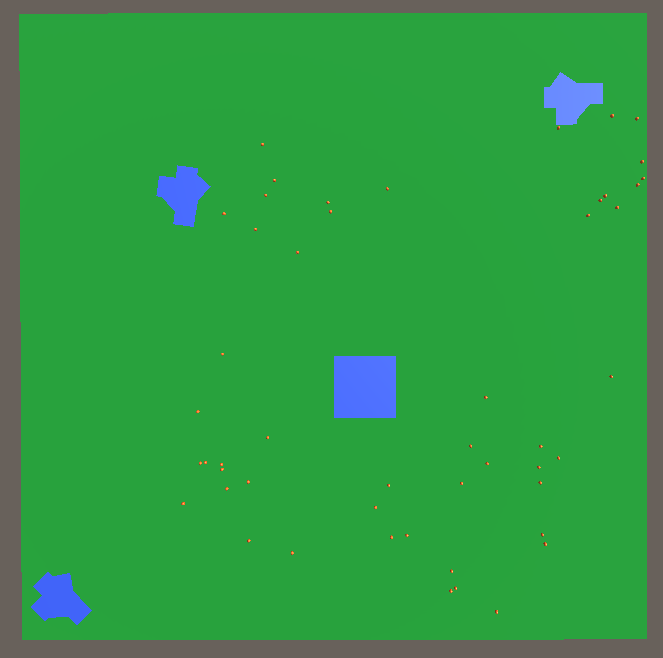
\includegraphics[width=7cm]{Images/Area_Simulation_7_only_rabbits_lot_of_food.png}
    \caption{Distribution of environmental components for Simulation 1.}
    \label{fig:simulation1EnvLayout}
\end{figure}

\subsection{Results}

\begin{figure}[H]
    \centering
    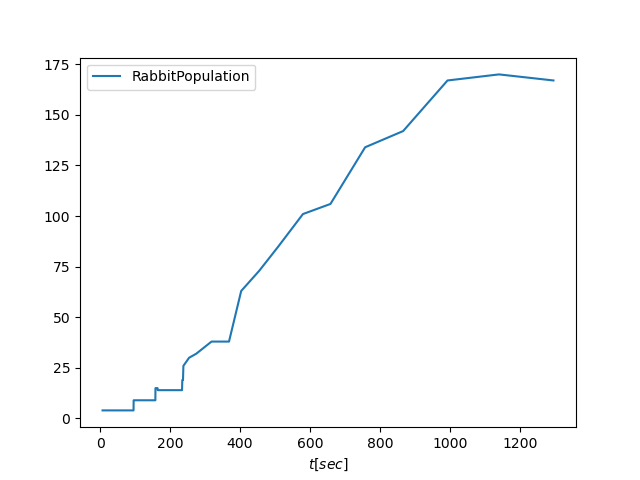
\includegraphics[width=0.9\textwidth]{Images/SimulationResults/Simulation_7_RabbitPopulation.png}
    \caption{Population of rabbits over time.}
    \label{fig:simulation1RabbitPopulation}
\end{figure}

\begin{figure}[H]
    \centering
    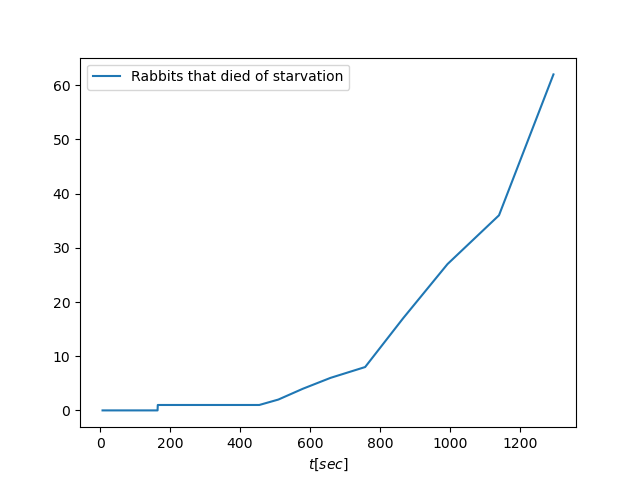
\includegraphics[width=0.9\textwidth]{Images/SimulationResults/Simulation_7_Rabbits that died of starvation.png}
    \caption{Number of rabbits that died of starvation over time.}
    \label{fig:simulation1RabbitsDiedOfHunger}
\end{figure}

\subsection{Analysis}
\subsubsection{Population}
As might be expected, in an environment ideal for rabbits to thrive, their numbers grew rapidly until the number of carrots in the environment was no longer sufficient for the rabbits to survive, then their numbers remained constant. 

\subsubsection{Features}

The graphs of the features over time were not very extensive, their values did not change, so only their final values are worth analysing. The median features of the rabbits at the end of simulation were as follows:
\begin{itemize}
    \item Speed: 74
    \item Sensory range: 85
    \item Fertility: 36
\end{itemize}

As we can see, the value of the fertility feature is not high, from which we can conclude that rapid reproduction was not crucial in this scenario. The speed was quite high, the faster the rabbits could get to the carrots the better chance they had that no other individual would eat it before him. It is interesting to note that the size of the sensor range is really large, despite the fact that in this case the rabbits did not derive any benefit from it because there were no foxes in the environment. The reason could be that there was not much generation of agents in such a one, old rabbits that had an unfavourable trait value in these conditions survived anyway, passing on their genes to their offspring.

\section{Simulation 2}
In this scenario, as in the previous one, there are no predators, but the amount of food is much lower, so that the rabbits will have to compete among themselves for resources in order to survive.
\subsection{Initial state of the environment}
\begin{description}
    \item[Number of agents]: 6 (3 male rabbits, 3 female rabbits)
    \item[Number of food generators]: 1, but with changed parameters:
    \begin{itemize}
        \item spawn interval: 10, instead of 8
        \item spawning radius: 15, instead of 10
        \item plant limit 20: instead of 10
    \end{itemize}
\end{description}

\begin{figure}[H]
    \centering
    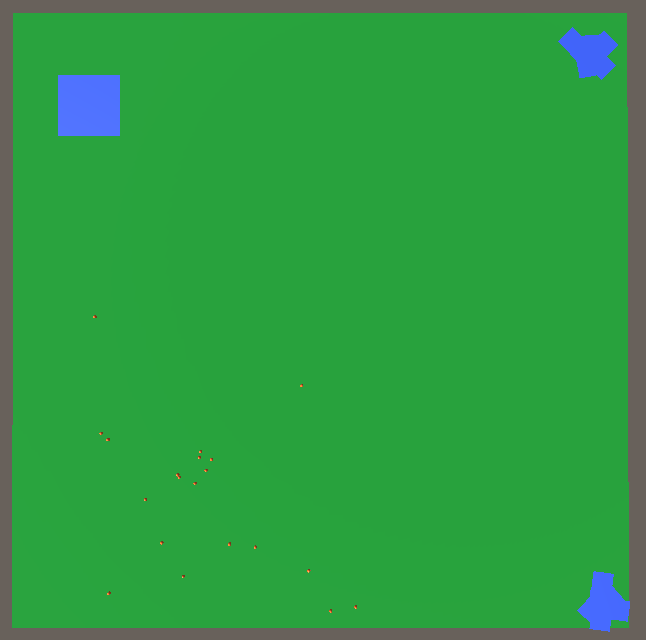
\includegraphics[width=7cm]{Images/Area_Simulation_4_small_amount_of_food.png}
    \caption{Distribution of environmental components for Simulation 2.}
    \label{fig:simulation2EnvLayout}
\end{figure}
    
\subsection{Results}

\begin{figure}[H]
    \centering
    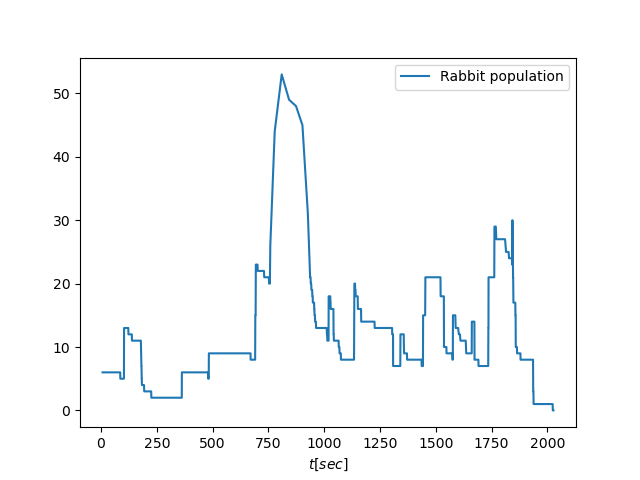
\includegraphics[width=0.9\textwidth]{Images/SimulationResults/Simulation_4_Rabbit population.png}
    \caption{Population of rabbits over time.}
    \label{fig:simulation2RabbitPopulation}
\end{figure}

\begin{figure}[H]
    \centering
    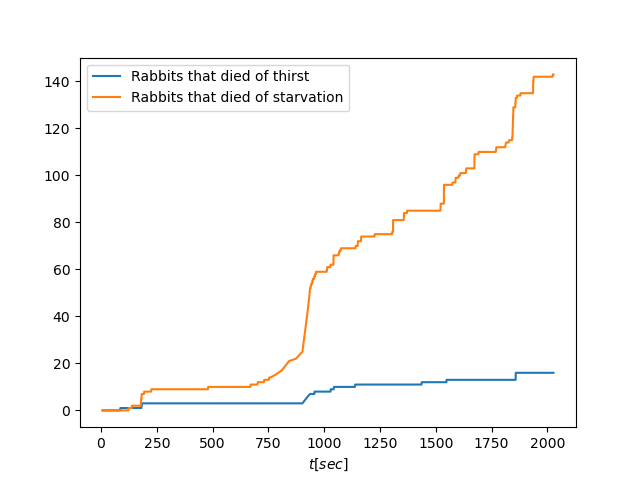
\includegraphics[width=0.9\textwidth]{Images/SimulationResults/Simulation_4_Rabbits that died of thirst_Rabbits that died of starvation.png}
    \caption{Death cause.}
    \label{fig:simulation2RabbitsDiedOfHunger}
\end{figure}

\begin{figure}[H]
    \centering
    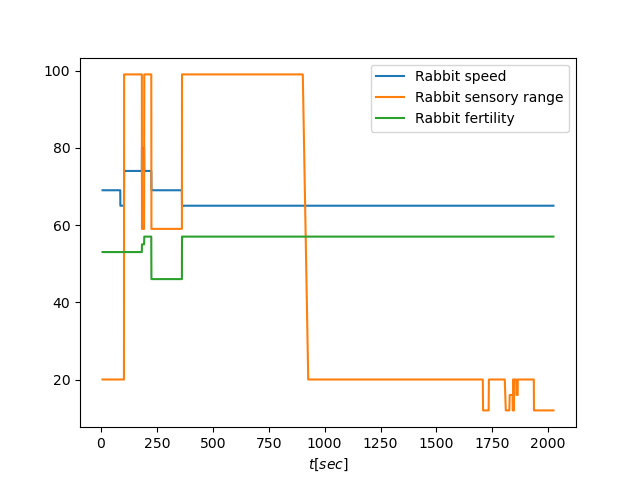
\includegraphics[width=0.9\textwidth]{Images/SimulationResults/Simulation_4_Rabbit speed_Rabbit sensory range_Rabbit fertility.png}
    \caption{Median value of features over time.}
    \label{fig:simulation2FeaturesMedian}
\end{figure}

\subsection{Analysis}
\subsubsection{Population}
In this scenario, initially the rabbits also reproduced rapidly, as can be seen with a maximum at around 800 seconds. At this point, however, the food ran out and the rabbits began to die out just as quickly, as can also be clearly seen in \autoref{fig:simulation2RabbitsDiedOfHunger}. Thereafter, their population fluctuated erratically until there were enough rabbits to eat almost all the food again, leading to the extinction of the entire species.

\subsubsection{Death causes}
As might be expected, most deaths were due to starvation. It is possible to note a sharp rise around the 900th second, corresponding to the extinction of a large proportion of rabbits, after the supply of carrots was no longer sufficient for the growing rabbit population. Thereafter, the function of deceased rabbits over time was linear, corresponding to a period of fluctuation in the rabbit population until the whole species became extinct.

\subsubsection{Features}
Unlike the previous scenario, in this case the rotation of individuals was much higher, allowing for better evolution of traits. Their final values were as follows:
\begin{itemize}
    \item Speed: 65
    \item Sensory range: 12
    \item Fertility: 57
\end{itemize}
The values for speed and fertility seem to be a quite reasonable compromise, reaching values sufficient for survival in the environment, but not too high to justify the high energy consumption that a high value for these traits brings. Whereas the sensory range value, as expected, is low, because in this scenario it does not bring any benefit to the rabbits, but only results in higher energy consumption.

\section{Simulation 3}
In this scenario, the amount of food is at a comfortable level for the rabbits, but there are predators in the environment that prey on them.
\subsection{Initial state of the environment}
\begin{description}
    \item[Number of agents]: 10 (4 male rabbits, 4 female rabbits, 1 male fox, 1 female fox)
    \item[Number of food generators]: 5
\end{description}

\begin{figure}[H]
    \centering
    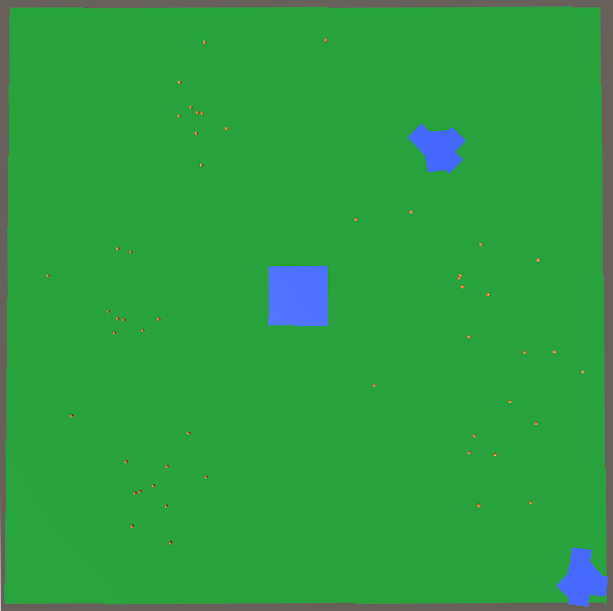
\includegraphics[width=7cm]{Images/Area_Simulation_5_and_6_with_foxes.png}
    \caption{Distribution of environmental components for Simulation 3 and 4.}
    \label{fig:simulation3EnvLayout}
\end{figure}
    
\subsection{Results}

\begin{figure}[H]
    \centering
    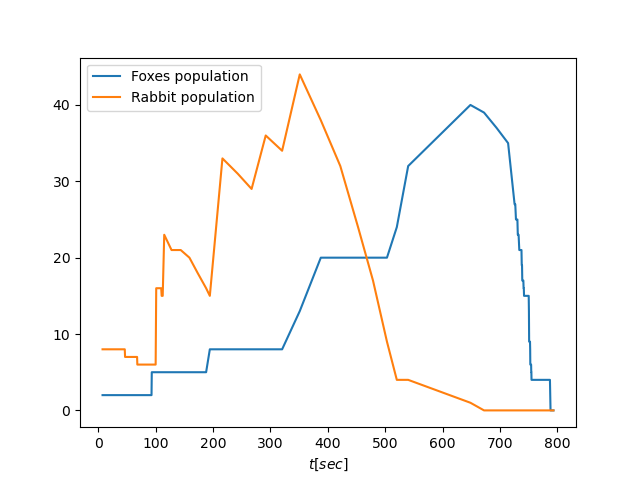
\includegraphics[width=0.9\textwidth]{Images/SimulationResults/Simulation_5_Foxes population_Rabbit population.png}
    \caption{Populations of agents over time.}
    \label{fig:simulation3Pupulations}
\end{figure}

\begin{figure}[H]
    \centering
    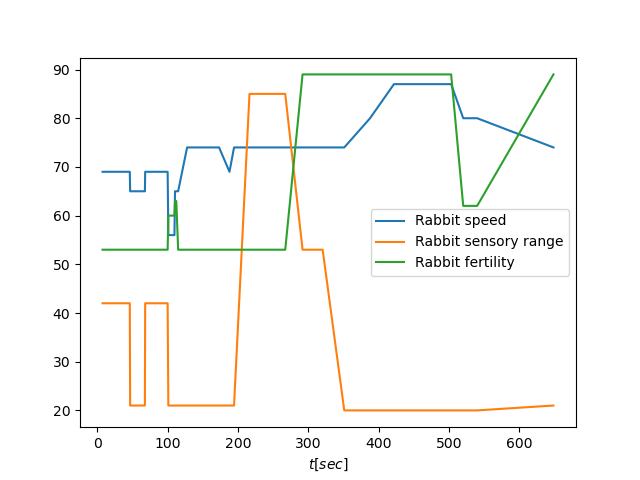
\includegraphics[width=0.9\textwidth]{Images/SimulationResults/Simulation_5_Rabbit speed_Rabbit sensory range_Rabbit fertility.png}
    \caption{Median value of rabbit features over time.}
    \label{fig:simulation3RabbitFeaturesMedian}
\end{figure}

\begin{figure}[H]
    \centering
    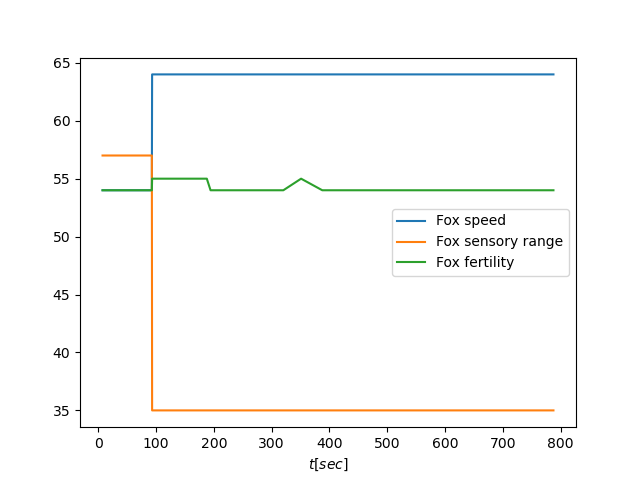
\includegraphics[width=0.9\textwidth]{Images/SimulationResults/Simulation_5_Fox speed_Fox sensory range_Fox fertility.png}
    \caption{Median value of fox features over time.}
    \label{fig:simulation3FoxFeaturesMedian}
\end{figure}

\begin{figure}[H]
    \centering
    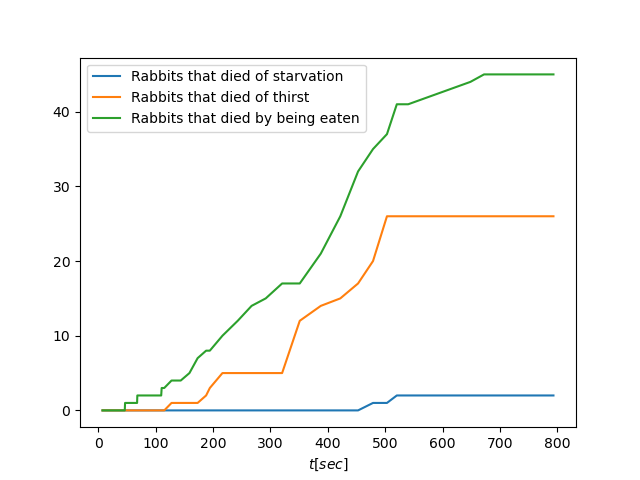
\includegraphics[width=0.9\textwidth]{Images/SimulationResults/Simulation_5_Rabbits that died of starvation_Rabbits that died of thirst_Rabbits that died by being eaten.png}
    \caption{Rabbits death cause.}
    \label{fig:simulation3RabbitDeathCause}
\end{figure}

\begin{figure}[H]
    \centering
    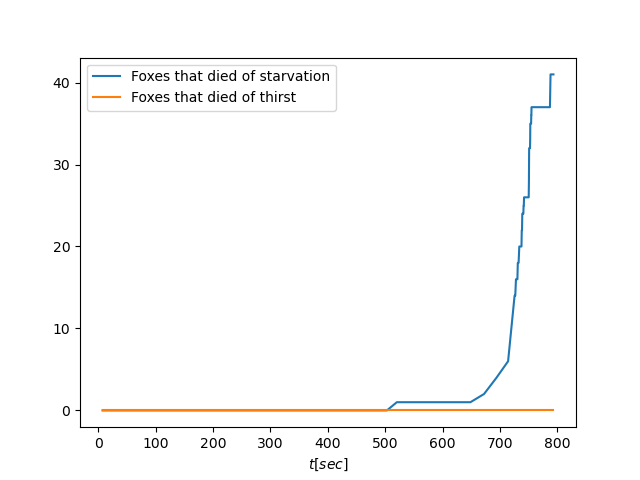
\includegraphics[width=0.9\textwidth]{Images/SimulationResults/Simulation_5_Foxes that died of starvation_Foxes that died of thirst.png}
    \caption{Foxes death cause.}
    \label{fig:simulation3FoxDeathCause}
\end{figure}

\subsection{Analysis}
\subsubsection{Population}
As in previous scenarios, the rabbit population initially shot up. But then, due to the fact that it was an ideal opportunity for the foxes to thrive as they had food and drink in abundance, the situation reversed. At around second 350, the fox population started to rise strongly, while the rabbit population fell very sharply. However, with this rapid growth, the foxes sealed their own fate, because it led to the extinction of the entire rabbit population. For a while, foxes with their needs satisfied multiplied even more, until they ran out of food and they, too, began to die out rapidly. So a strong correlation can be seen between the two species and how prosperity can easily turn into inhospitable conditions.

\subsubsection{Death causes}
Most rabbits were obviously eaten by foxes, but quite a few deaths were also caused by thirst. On the other hand, no fox died of thirst. This was most probably due to the fact that the foxes, by staying at the watering holes, scared away the rabbits, which were afraid to approach the predators. Therefore, the foxes not only actively contributed to the extinction of the rabbits by eating them, but also passively cut off their access to water.

\subsubsection{Features}
In the case of rabbits, we see dynamically changing feature values, actively striving towards the most favourable values for rabbits in this environment. The features that were more valuable to the rabbits were fertility, and speed, as can be seen when the values of these features reached very high scores in the later stages of the simulation. Interestingly, sensory range apparently did not give the rabbits enough of an advantage to make it profitable to bear its genetic cost. 

In contrast, for foxes, the values remained virtually the same throughout most of the simulations. This may be due to the fact that individuals of this species only started dying out towards the end, so the same genes were in the gene pool all the time. For the less adapted individuals, the environment was favourable enough for them to survive anyway, giving them the opportunity to pass on their weak genes to their offspring.

\newpage
\section{Simulation 4}
\label{Simulation4}
This scenario is no different from the previous one, but the simulation went differently.
\subsection{Initial state of the environment}
The environment is exactly the same as the previous one.

\subsection{Results}

\begin{figure}[H]
    \centering
    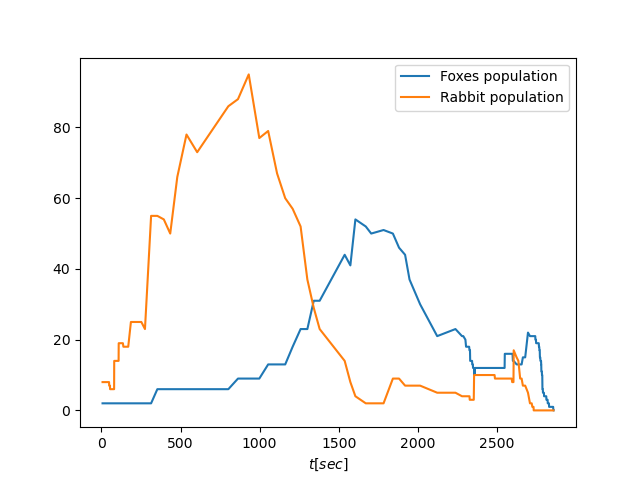
\includegraphics[width=0.9\textwidth]{Images/SimulationResults/Simulation_6_Foxes population_Rabbit population.png}
    \caption{Populations of agents over time.}
    \label{fig:simulation4Pupulations}
\end{figure}

\begin{figure}[H]
    \centering
    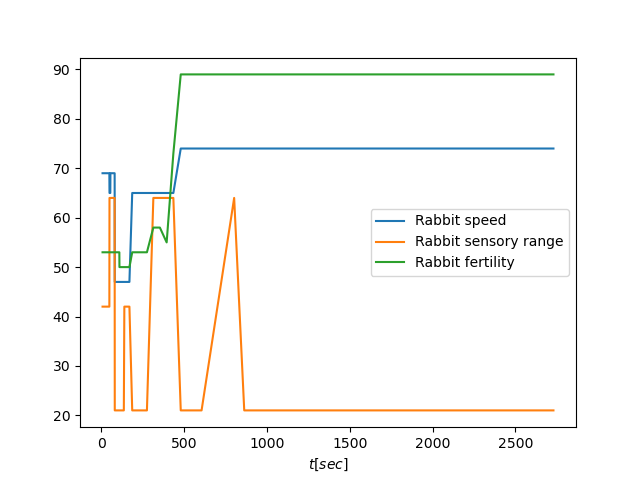
\includegraphics[width=0.9\textwidth]{Images/SimulationResults/Simulation_6_Rabbit speed_Rabbit sensory range_Rabbit fertility.png}
    \caption{Median value of rabbit features over time.}
    \label{fig:simulation4RabbitFeaturesMedian}
\end{figure}

\begin{figure}[H]
    \centering
    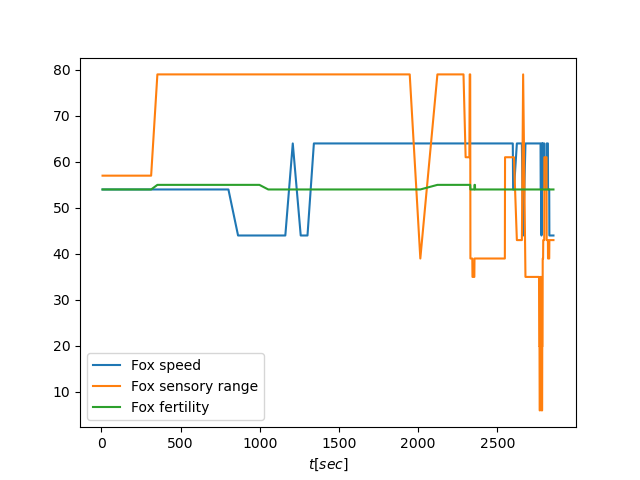
\includegraphics[width=0.9\textwidth]{Images/SimulationResults/Simulation_6_Fox speed_Fox sensory range_Fox fertility.png}
    \caption{Median value of fox features over time.}
    \label{fig:simulation4FoxFeaturesMedian}
\end{figure}

\begin{figure}[H]
    \centering
    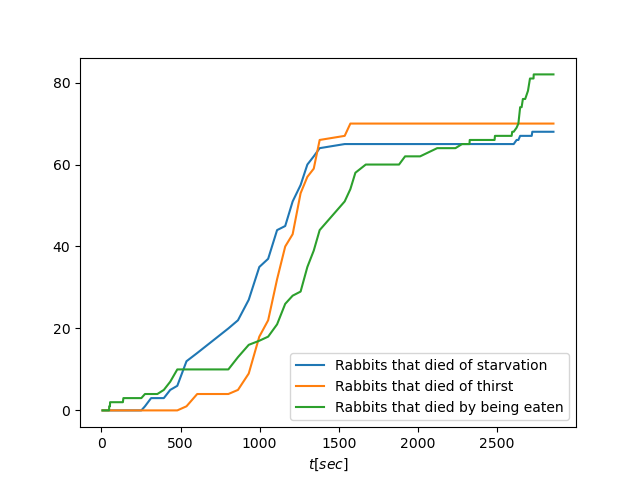
\includegraphics[width=0.9\textwidth]{Images/SimulationResults/Simulation_6_Rabbits that died of starvation_Rabbits that died of thirst_Rabbits that died by being eaten.png}
    \caption{Rabbits death cause.}
    \label{fig:simulation4RabbitDeathCause}
\end{figure}

\begin{figure}[H]
    \centering
    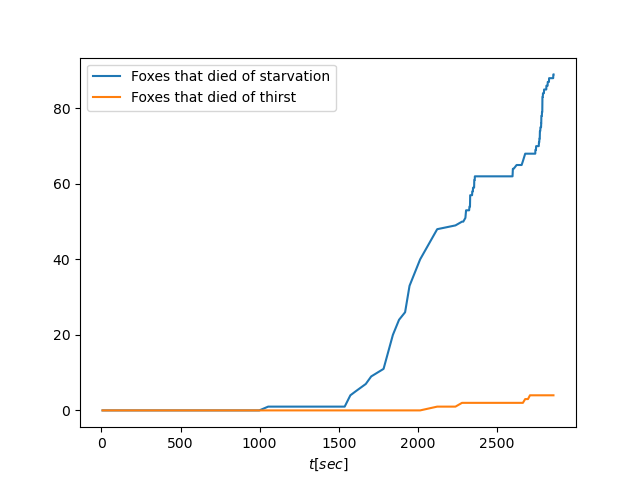
\includegraphics[width=0.9\textwidth]{Images/SimulationResults/Simulation_6_Foxes that died of starvation_Foxes that died of thirst.png}
    \caption{Foxes death cause.}
    \label{fig:simulation4FoxDeathCause}
\end{figure}

\subsection{Analysis}
\subsubsection{Population}
In this scenario, as in the previous one, once the foxes had eaten a large proportion of the rabbits, they themselves began to starve to death. However, this time a few rabbits managed to survive and multiply again, but the foxes quickly dealt with them, this time finally. However, a certain cyclicality can be observed, if the rabbits had started to breed later, more foxes would have died out and they could have rebuilt their population more by reaching the same environmental state as originally (however with different, more adapted trait values nonetheless).

\subsubsection{Death causes}
Because the leaves started reproducing later than in the previous simulation, this led to more deaths from starvation, which were previously much lower. This time it had values similar to death from thirst and being eaten by a predator. In this simulation the availability of carrots started to play a role again, there were not enough carrots in the environment to satisfy such a growing population of rabbits.

\subsubsection{Features}
The dominant feature values for rabbits were established at the very beginning, where the weakest individuals were immediately eaten by the foxes. This led to a state where rabbits had a genetic advantage over foxes for most of the simulations, which was most likely the reason that foxes reproduced more slowly than in the previous simulation. 

The features of foxes began to develop rapidly towards the end of the simulation, when foxes began to die out and only strong individuals could survive in this difficult environment. The final values of the features are as follows: 
\begin{itemize}
    \item Speed: 44
    \item Sensory range: 43
    \item Fertility: 54
\end{itemize}
Thus, it can be seen that for foxes each of the traits was important, but they could not afford their high values. 
\chapter{Conclusions} \label{chr:conclusions}

The objective set out in the introduction has been met. The tests conducted demonstrate that the developed modules operate as intended and can be used to perform the Winston-Lutz test and leaf alignment analysis.

The fact that the tools have been developed as part of a web application makes them highly accessible for use on any device with access to a modern browser. Moreover, the application's open-source nature opens up a wide range of possible applications in situations where it was previously impractical, frequently because of resource constraints.

However, it should be mentioned that the application is currently in the prototype stage and has not been certified. As such, it should not be applied to the calibration of medical equipment meant to be utilized during procedures on human beings. At this stage of development, the application is only a proof of concept. Nevertheless, it does demonstrate the potential of such solutions, which, with sufficient effort, could greatly facilitate the operation of numerous facilities utilising linear accelerators, given that such devices will require calibration regularly.

The analysis of the results of the W-L tests reveals that in instances where the test is expected to yield accurate results, it does so. Furthermore, in cases that should identify the machine as uncalibrated, results also match. This proves that the module has been correctly embedded in the application. 

Observing the analysis of the results for LA in an analogous way shows the correct implementation of the module, giving the expected results. Further interpretation, however, leads to the conclusion that the more complex the shape, the greater the problem the edge detection algorithm will have, which can lead to erroneous indications. 

The outcomes of the work has been reviewed by Damian Kubat, the head of the Department of Medical Physics at the National Institute of Oncology in Kraków. He provided a positive feedback on its implementation and indicates that it is a valuable tool, especially if developed further.

\chapter{Further development possibilities}
\label{furtherDevelopmentPossibilitiesChapter}
\section{Possible fields of application}
\begin{itemize}
    \item Computer games - fauna, realistic backgrounds that enhance gameplay and immersion
    \item More advanced simulations that need agents who realistically make decisions based on their needs
    \item Background for various types of animation
    \item Scientific research - modelling the actual ecosystem
\end{itemize}

\section{Technicalities and improvement to implementation}
\begin{description}
    \item[Fuzzy systems for switching states] - Instead of the current ranking system, fuzzy logic could be used, which seems a very good solution for this type of task. The state switching system itself would also become clearer and more consistent.
\end{description}

\section{New features}
\begin{description}
    \item[Size] - Influences strength and noticeability. Reduces the risk of attack by birds (they will not be able to carry the prey), but increases by foxes (larger animals give more energy).
\end{description}

\section{New mechanics}
\begin{description}
    \item[Pregnancy] - add a pregnancy period after mating interaction that offspring is spawned after. This will add another layer of complexity, as a pregnant rabbit may be eaten before its offspring are born.
    \item[Aging of agents] - This is linked to the pregnancy mechanic, the agents would have different stages of development. Right after birth, young versions of agents would be spawned, with temporarily lowered trait values, unable to reproduce, or maybe even using slightly less trained policies to reflect their lesser experience in all activities.
    \item[Camoflage] - extension of the spotting system, could significantly enhance the simulation and mechanics of hunting.
    \item[Attack sytem] - another extension to hunting mechanic. Agents would have health points, and predators would have to first kill animal to be able to eat it.
    \item[Dying of plants] - After a while the plant would wither and die. It would be possible to get rid of the parameter of the maximum number of plants around the generator, because the maximum number of plants would stabilise and remain naturally at a certain level, when the frequency of death of old plants would equal the frequency of appearance of new ones.
    \item[Better plant growth model] - plants will grow differently depending on their position in the environment, for example they will grow better near water.
\end{description}

\section{New States}
\begin{description}
    \item[Better chilling] - add some agent behavior to chilling state
    \item[Sleeping] - add sleeping state that agent reduces tiredness and regenerates itself
    \item[Dead] - instead of disappearing immediately after death, the bodies of agents could remain in the environment for some time
\end{description}

\section{New Species}
\begin{description}
    \item[Hawk] - eats rabbits. Reproduces through laying down eggs that can be eaten by foxes (but it would give much less energy than rabbit, so foxes would rather hunt for them), so reproduction for hawks would be more challenging than for rabbits, for example. Hawks could only eat small rabbits, so this feature would be more relevant. This species, however, would have their own unique characteristics that could give them an advantage in certain environments, such as flying (their movement would not be restricted by environmental elements and they could spot prey more easily and the prey would be less likely to escape).
    \item[Scavenging species] - eats dead agents
    \item[Omnivorous species] - eats other agents and plants
\end{description}

\addcontentsline{toc}{chapter}{Bibliography}
\bibliographystyle{plain}
\bibliography{Bibliography}

\appendix
\chapter{Training files}
\label{TrainingFiles}
\section{Configuration Files}
The following are the configuration in yaml format used in the ML-Agents toolkit.

The individual files differ only in the values of the rewards and the size of the test environment (in hunting and escaping, other models use one from common configuration), the other parameters are the same for each test environment and are shown once in common section below.
\\
\\
The meaning of each parameter is described in the documentation for the ML-Agents toolkit \cite{MLAgentsParameterDescription}.

\subsection{Common Configuration}
\begin{lstlisting}
behaviors:
  AgentMovement:
    trainer_type: ppo
    hyperparameters:
      batch_size: 1024
      buffer_size: 10240
      learning_rate: 0.0003
      beta: 0.005
      epsilon: 0.2
      lambd: 0.95
      num_epoch: 3
      learning_rate_schedule: linear
    network_settings:
      normalize: false
      hidden_units: 256
      num_layers: 1
      vis_encode_type: simple
    reward_signals:
      extrinsic:
        gamma: 0.99
        strength: 1.0
    keep_checkpoints: 5
    max_steps: 1000000
    time_horizon: 64
    summary_freq: 10000
environment_parameters:
  is_training: 1

  # features
  agent_speed:
    sampler_type: uniform
    sampler_parameters:
      min_value: 0
      max_value: 100
  agent_sensory_range:
    sampler_type: uniform
    sampler_parameters:
      min_value: 0
      max_value: 100
      
  # training area size
  training_area_size:
    curriculum:
      - name: SmallAreaSize
        completion_criteria:
          measure: progress
          behavior: AgentMovement
          min_lesson_length: 5
          threshold: 0.1
        value: 0.5
      - name: MediumAreaSize
        completion_criteria:
          measure: progress
          behavior: AgentMovement
          min_lesson_length: 5
          threshold: 0.4
        value: 1.0
      - name: LargeAreaSize
        completion_criteria:
          measure: progress
          behavior: AgentMovement
          min_lesson_length: 5
          threshold: 0.7
        value: 2.0
      - name: ExtraLargeAreaSize
        value: 3.0
\end{lstlisting}

\subsection{Drinking Configuration}
\begin{lstlisting}
environment_parameters:
  rabbit_each_episode_fixed: -1.0
  fox_each_episode_fixed: -1.0
  agent_bump_into_wall: -0.2
  agent_bump_into_food: -0.2
  agent_drink_reward: 1.0
\end{lstlisting}

\subsection{Eating Carrot Configuration}
\begin{lstlisting}
environment_parameters:
  rabbit_eating_carrot_reward: 1
  rabbit_each_episode_fixed: -1
  agent_bump_into_wall: -0.2
    agent_bump_into_water: -0.2
\end{lstlisting}

\subsection{Mating Configuration}
\begin{lstlisting}
environment_parameters:
  rabbit_each_episode_fixed: -1
  fox_each_episode_fixed: -1
  agent_bump_into_wall: -0.01
  agent_bump_into_water: -0.01
  agent_bump_into_food: -0.01
  rabbit_mating_reward: 1
  fox_mating_reward: 1
\end{lstlisting}

\subsection{Hunting Configuration}
\begin{lstlisting}
environment_parameters:
  # rewards
  fox_eating_rabbit_reward: 1
  fox_each_episode_fixed: -1
  agent_bump_into_wall: -0.01
  agent_bump_into_water: -0.01
  agent_bump_into_food: -0.01

  # training area size
  training_area_size:
    curriculum:
      - name: SmallAreaSize
        completion_criteria:
          measure: progress
          behavior: FoxMovement
          min_lesson_length: 5
          threshold: 0.15
        value: 1.0
      - name: MediumAreaSize
        completion_criteria:
          measure: progress
          behavior: FoxMovement
          min_lesson_length: 5
          threshold: 0.5
        value: 1.0
      - name: LargeAreaSize
        completion_criteria:
          measure: progress
          behavior: FoxMovement
          min_lesson_length: 5
          threshold: 0.75
        value: 1.0
      - name: ExtraLargeAreaSize
        value: 1.0
\end{lstlisting}

\subsection{Escaping Configuration}
\begin{lstlisting}
environment_parameters:
  # rewards
  rabbit_each_episode_fixed: 1
  rabbit_on_eaten: -1
  agent_bump_into_wall: -0.01
  agent_bump_into_water: -0.01
  agent_bump_into_food: -0.01

  # training area size
  training_area_size: 1.0
\end{lstlisting}

\section{Results}
The graphs were created using the TensorBoard tool. \cite{TensorboardTool}

\begin{figure}[H]
    \centering
    \includegraphics[width=\textwidth]{Images/result_drinking_v2.png}
    \caption{Results of training Drinking model.}
    \label{fig:drinkingTrainingResults}
\end{figure}

\begin{figure}
    \centering
    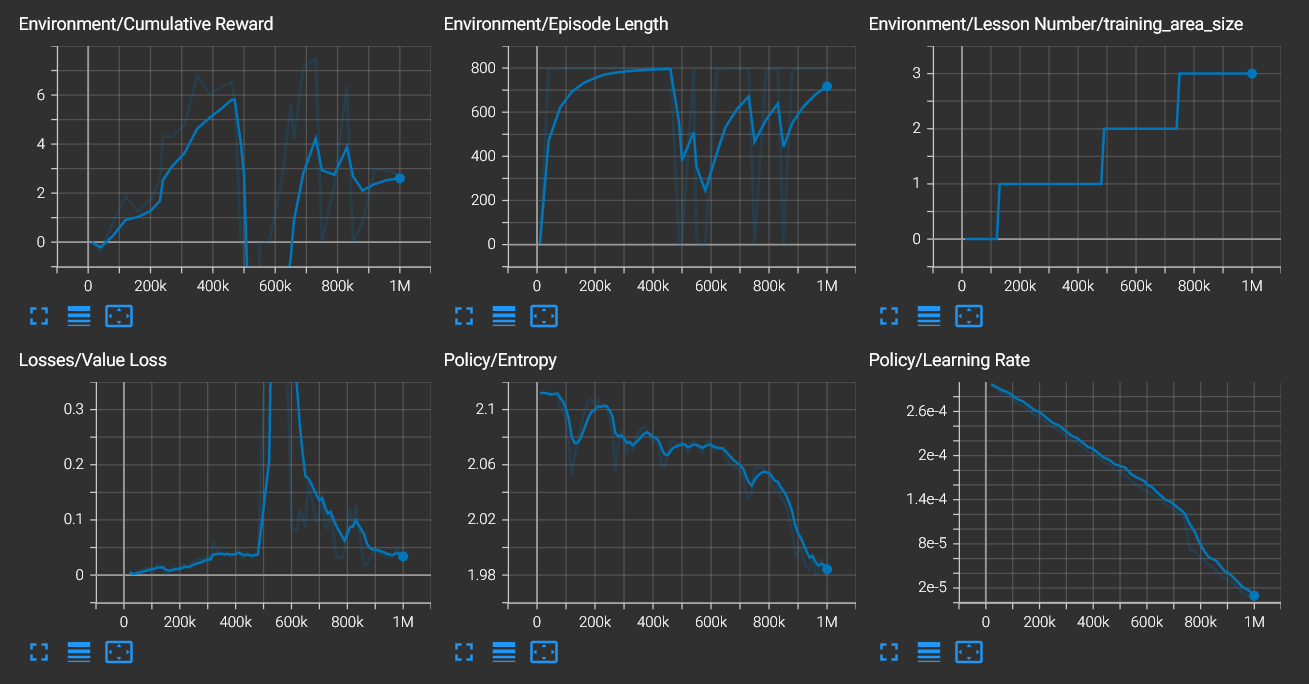
\includegraphics[width=\textwidth]{Images/result_eating_v2.png}
    \caption{Results of training EatingCarrot model.}
    \label{fig:eatingCarrotTrainingResults}
\end{figure}

\begin{figure}
    \centering
    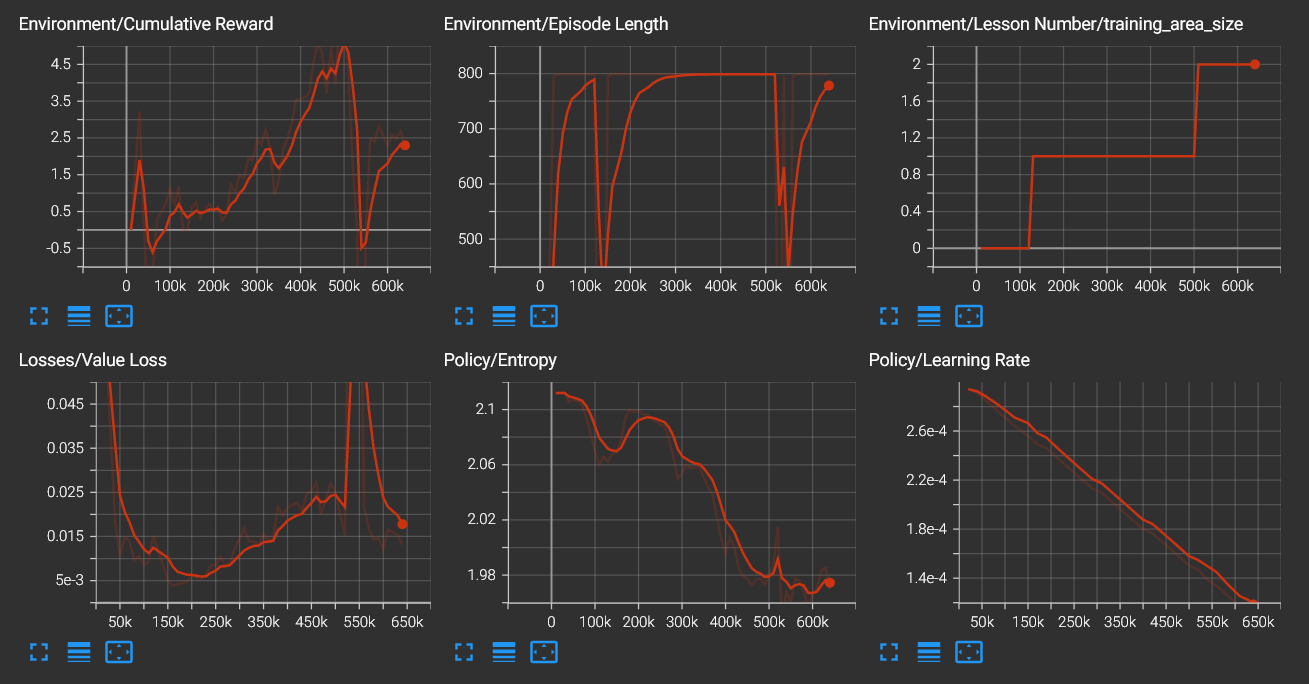
\includegraphics[width=\textwidth]{Images/result_mating_rabbit_v2.png}
    \caption{Results of training Mating-Rabbit model.}
    \label{fig:matingRabbitTrainingResults}
\end{figure}

\begin{figure}
    \centering
    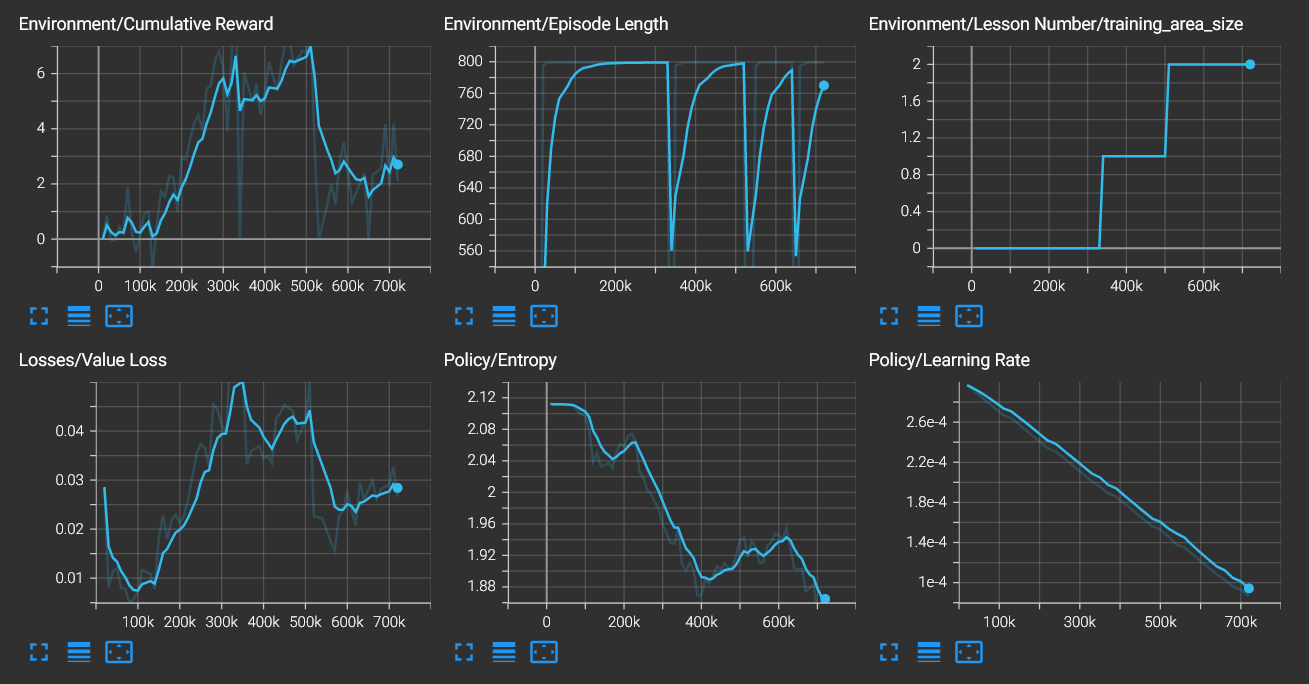
\includegraphics[width=\textwidth]{Images/result_mating_fox_v2.png}
    \caption{Results of training Mating-Fox model.}
    \label{fig:matingFoxTrainingResults}
\end{figure}

\begin{figure}
    \centering
    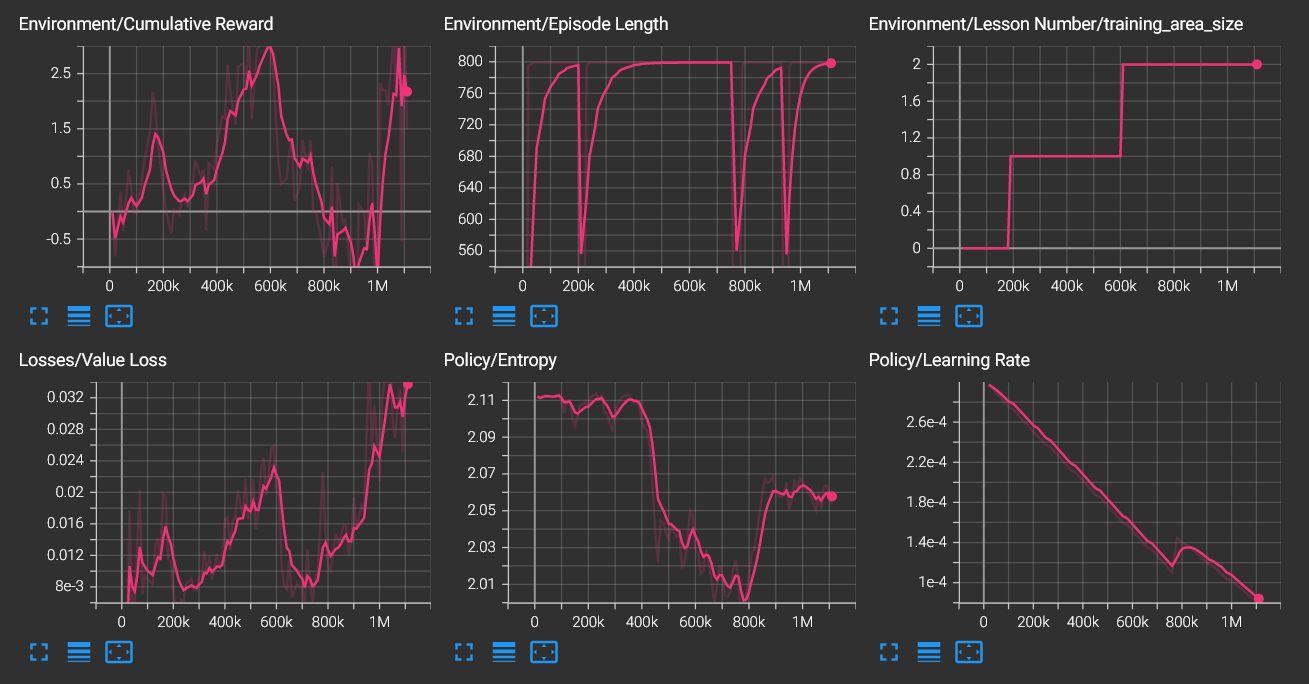
\includegraphics[width=\textwidth]{Images/result_hunting_v2.png}
    \caption{Results of training Hunting model.}
    \label{fig:huntingTrainingResults}
\end{figure}

\begin{figure}
    \centering
    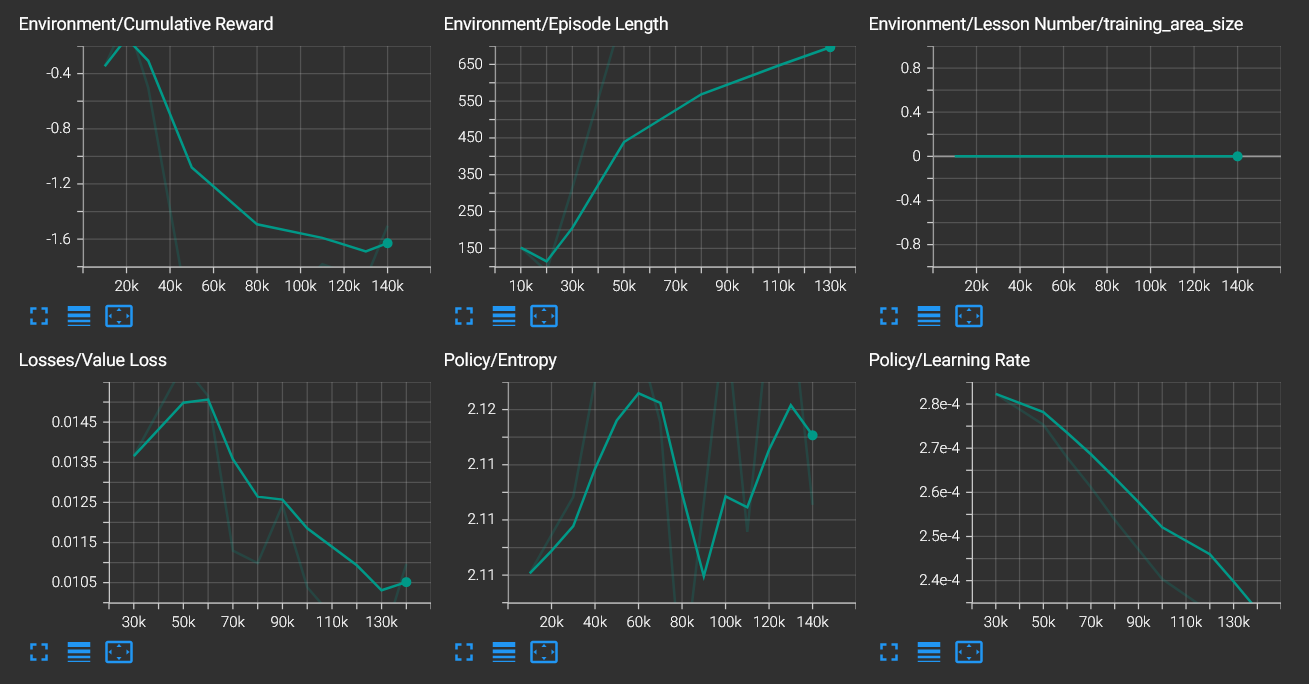
\includegraphics[width=\textwidth]{Images/result_escaping_v2.png}
    \caption{Results of training Escaping model.}
    \label{fig:escapingTrainingResults}
\end{figure}
\chapter{Packages and Versions} \label{chr:packagesAndVersions}
This section describes tools and packages used in the application, broken down into a backend, where the server and technologies needed for image analysis are included, and a frontend, where the tools needed for display UI are included.

\section*{Frontend}

\begin{description}

    \item[Nodejs] 20
    \begin{itemize}
        \item \url{https://nodejs.org/en}
    \end{itemize}

    \item[Typescript] 5.2.2
    \begin{itemize}
        \item \url{https://www.typescriptlang.org/}
        \item \url{https://www.npmjs.com/package/typescript/v/5.2.2}
    \end{itemize}

    \item[React] 18.2.0
    \begin{itemize}
        \item \url{https://react.dev/}
        \item \url{https://www.npmjs.com/package/react/v/18.2.0}
    \end{itemize}

    \item[React Router] 6.16.0
    \begin{itemize}
        \item \url{https://reactrouter.com/en/main}
        \item \url{https://www.npmjs.com/package/react-router-dom/v/6.16.0}
    \end{itemize}

    \item[Tanstack React Query] 4.35.3
    \begin{itemize}
        \item \url{https://tanstack.com/query/v4}
        \item \url{https://www.npmjs.com/package/@tanstack/react-query/v/4.35.3}
    \end{itemize}

    \item[Axios] 1.5.0
    \begin{itemize}
        \item \url{https://github.com/axios/axios}
        \item \url{https://www.npmjs.com/package/axios/v/1.5.0}
    \end{itemize}

    \item[daisyUI] 3.7.6
    \begin{itemize}
        \item \url{https://v3.daisyui.com/}
        \item \url{https://www.npmjs.com/package/daisyui/v/3.7.6}
    \end{itemize}

    \item[tailwindcss] 3.3.3
    \begin{itemize}
        \item \url{https://tailwindcss.com/}
        \item \url{https://www.npmjs.com/package/tailwindcss/v/3.3.3}
    \end{itemize}

\end{description}

\section*{Backend}

\begin{description}

    \item[Python] 3.11
    \begin{itemize}
        \item \url{https://www.python.org/}
    \end{itemize}

    \item[Django] 4.2.5
    \begin{itemize}
        \item \url{https://www.djangoproject.com/}
        \item \url{https://pypi.org/project/Django/4.2.5/}
    \end{itemize}

    \item[Django REST framework] 3.14.0
    \begin{itemize}
        \item \url{https://www.django-rest-framework.org/}
        \item \url{https://pypi.org/project/djangorestframework/3.14.0/}
    \end{itemize}

    \item[Daphne] 4.0.0
    \begin{itemize}
        \item \url{https://github.com/django/daphne}
        \item \url{https://pypi.org/project/daphne/4.0.0/}
    \end{itemize}

    \item[Pylinac] 3.23.2
    \begin{itemize}
        \item \url{https://pylinac.readthedocs.io/en/release-v3.23}
        \item \url{https://pypi.org/project/pylinac/3.23.2/}
    \end{itemize}

    \item[Pydicom] 2.4.4
    \begin{itemize}
        \item \url{https://pydicom.github.io/pydicom/stable/}
        \item \url{https://pypi.org/project/pydicom/2.4.4/}
    \end{itemize}

    \item[OpenCV] 4.10.0
    \begin{itemize}
        \item \url{https://opencv.org/}
        \item \url{https://pypi.org/project/opencv-python/4.10.0.84/}
    \end{itemize}

    \item[NumPy] 1.26.4
    \begin{itemize}
        \item \url{https://numpy.org/}
        \item \url{https://pypi.org/project/numpy/1.26.4/}
    \end{itemize}

\end{description}


\end{document}
%% ------------------------------------------------------------------